% ============================================================================
%  The Polyglot's Shorthand -- Technical Whitepaper
%  Compile:  pdflatex whitepaper && pdflatex whitepaper   (or: latexmk -pdf)
%  Engine:   pdfLaTeX (emoji are written as named placeholders, see \emo)
% ============================================================================
\documentclass[11pt,a4paper]{article}

% ---------------------------------------------------------------- packages --
\usepackage[T1]{fontenc}
\usepackage[utf8]{inputenc}
\usepackage{lmodern}
\usepackage[margin=2.4cm]{geometry}
\usepackage{microtype}
\usepackage{amsmath,amssymb,amsthm,bm}
\usepackage{booktabs,tabularx,multirow}
\usepackage[table]{xcolor}
\usepackage{graphicx}
\usepackage{tikz}
\usetikzlibrary{arrows.meta,positioning,fit,calc,backgrounds}
\usepackage{pgfplots}
\pgfplotsset{compat=1.17}
\usepackage{algorithm}
\usepackage[noend]{algpseudocode}
\usepackage{caption}
\usepackage{enumitem}
\usepackage{listings}
\usepackage[colorlinks=true,linkcolor=accent,citecolor=accent,urlcolor=accent]{hyperref}
\usepackage[nameinlink,capitalise]{cleveref}

% ------------------------------------------------------------------ styling --
\definecolor{accent}{RGB}{31,78,121}
\definecolor{accentlight}{RGB}{214,228,240}
\definecolor{warn}{RGB}{176,58,46}
\definecolor{okgreen}{RGB}{39,119,72}
\definecolor{muted}{RGB}{110,110,110}
\captionsetup{font=small,labelfont={bf,color=accent}}
\setlist{nosep,leftmargin=1.4em}
\lstset{basicstyle=\ttfamily\small,columns=fullflexible,frame=single,
        rulecolor=\color{muted!40},backgroundcolor=\color{accentlight!35},
        xleftmargin=0.5em,xrightmargin=0.5em}

\newtheorem{definition}{Definition}
\newtheorem{proposition}{Proposition}
\theoremstyle{remark}
\newtheorem*{remark}{Remark}

% ------------------------------------------------------------------- macros --
\newcommand{\lbl}[1]{\texttt{#1}}                      % class label
\newcommand{\hi}[1]{\textit{#1}}                       % Hinglish text
\newcommand{\emo}[1]{\textsf{\small$\langle$#1$\rangle$}} % emoji placeholder
\newcommand{\R}{\mathbb{R}}
\newcommand{\x}{\bm{x}}
\newcommand{\W}{\bm{W}}
\newcommand{\bb}{\bm{b}}
\newcommand{\z}{\bm{z}}
\newcommand{\p}{\bm{p}}
\DeclareMathOperator*{\argmin}{arg\,min}
\DeclareMathOperator*{\argmax}{arg\,max}
\DeclareMathOperator{\softmax}{softmax}
\DeclareMathOperator{\CE}{CE}
\DeclareMathOperator{\KL}{KL}
\DeclareMathOperator{\LN}{LN}
\DeclareMathOperator{\GELU}{GELU}
% confusion-matrix cell: \cm{shade 0-100}{count}
\newcommand{\cm}[2]{\cellcolor{accent!#1}\ifnum#1>45\color{white}\fi#2}

% ----------------------------------------------------------------- metadata --
\title{\vspace{-1.2em}\textbf{The Polyglot's Shorthand}\\[0.3em]
  \large A Hashed Sparse Multi-Head Classifier for Intent and Sentiment\\
  in Romanized Hindi--English Customer-Support Text\\[0.4em]
  \normalsize\color{muted}Technical Whitepaper\\[0.2em]
  }
\author{Harsh Raj - B25352 - General Engineering}
\date{September 2026}

% ============================================================================
\begin{document}
\maketitle

\begin{abstract}
\noindent
Customer-support messages in India are frequently written in \emph{Romanized
code-mixed} Hindi--English (``Hinglish''): non-standard spelling, texting
shorthand (\hi{nhi}, \hi{kr}, \hi{plz}), English loanwords and emoji that can
invert the literal polarity of a sentence. We present a compact, fully
reproducible reference system that maps such a message to one of six
support \emph{intents} and one of three \emph{sentiment} classes, together
with calibrated confidences and a human-review flag. The system combines a
\textbf{Unicode-preserving normalizer}, eight \textbf{prefixed feature channels} (word and
character $n$-grams, a shorthand-alias channel, and symbol$\times$word
interaction features), \textbf{CRC32 feature hashing} into $D=2^{15}$ buckets, and two
\textbf{softmax heads }trained jointly by \textbf{class-balanced stochastic gradient descent}.
Post-hoc temperature scaling and a coverage-maximizing selective-prediction
threshold are fitted on a validation split. The complete model has
\textbf{294{,}921 parameters} (1.13\,MiB as float32; 106\,KB compressed), depends only
on NumPy, and serves a request in \textbf{0.218ms at the 95th percentile} on a
laptop CPU. On a leakage-controlled, group-split synthetic benchmark the
system reaches an \textbf{intent macro-F1 of $0.820$} (group-bootstrap 95\% CI
$[0.568, 0.960]$) but a \textbf{sentiment macro-F1 of only $0.423$,} with zero recall
on held-out positive messages and zero of five sarcasm contrast pairs solved.
We evaluate the system through ablations, stress tests under unseen misspellings, calibration
error, hash-collision statistics and a qualitative error analysis, and we
argue explicitly which of the problem's robustness claims are \emph{not}
established by this evidence.

\smallskip\noindent
\textbf{Version 1.1.} Building on the v1.0 finding that positive affect
existed only inside \lbl{feedback}, we (i)~\textbf{enrich the benchmark from 96 to 213
seeds} (221 to 884 rows) with \textbf{positive, negative and neutral affect} in
\emph{every} intent, and (ii)~add a NumPy \textbf{self-attention branch} with
hand-derived gradients and combine its logits with those of the linear model. On the
regenerated 190-row development test, the v1.1 \lbl{full} model reaches \textbf{intent
macro-F1 $0.901$ $[0.782, 0.970]$ and sentiment macro-F1 $0.845$
$[0.718, 0.944]$, with positive recall $0.72$} and 9 of 12 sarcasm pairs solved.
A linear-only model trained on the same enriched data scores $0.860$ and
$0.810$, so most of the sentiment gain comes from data and a smaller, paired
improvement comes from attention. The model has \textbf{827{,}721 parameters and a p95
latency of 0.427\,ms}. The small frozen audit set regresses from 3 to 6 errors
(\cref{sec:v11}).

\smallskip\noindent
\textbf{Version 1.2.} We separate pretrained knowledge from new data and then
distil. On the exact v1.1 splits, a pretrained Hinglish encoder
\textbf{(hing-roberta-mixed, 278M parameters)} trained only on the v1.1 training split
fixes sentiment (paired $+0.159$ $[+0.056, +0.282]$) but not intent. Adding
1{,}202 generated support messages, 2{,}323 augmented variants and 4{,}000
public tweets (teacher~v2) reaches \textbf{intent $0.966$ }$[0.92, 0.99]$ and solves 29
of 40 pairs in a new hand-written contrast set (v1.1: 10). We then use its soft labels on
\textbf{66{,}166 sentences} train an \textbf{11.88M-parameter student} that keeps the v1.1
hashed pieces, adds four pre-LN Transformer blocks and runs without PyTorch
(ONNX INT8; p95 0.81\,ms, 4.29\,ms at 512 code points). \textbf{The student does
\emph{not} keep the teacher's gains.} Its intent $0.914$ and sentiment $0.916$
cannot be cleanly resolved against v1.1, and sentiment is significantly below teacher~v2
($-0.092$ $[-0.184, -0.020]$). Distillation is not shown to help over a no-KD
student, and sentiment varies across seeds (sd $0.049$). Every evaluation set
remains LLM-generated (\cref{sec:v12}).

\smallskip\noindent
\textbf{Availability.} The source, the released checkpoints and both front
ends are at \url{https://github.com/HarshRaj4343/Polyglots-Shorthand}. A
hosted demo of the deployed student, with every model of this paper
selectable, runs at \url{https://polyglots-shorthand.onrender.com/}
(\cref{sec:v12hosted}).
\end{abstract}

\tableofcontents
\vspace{1em}\hrule

% ============================================================================
\section{Introduction}
\label{sec:intro}

Code-mixing i.e alternating between two or more languages inside a single
utterance,is the default register of informal Indian digital
communication. When Hindi is written in Latin script
there is no orthographic standard: \hi{nahi}, \hi{nhi}, \hi{nai} and
\hi{nahii} all denote the same negator, and spelling varies by region,
keyboard and individual. Benchmarks such as \textbf{GLUECoS}
and \textbf{SemEval-2020} Task~9 show that these properties
degrade models built for monolingual, standardized text.

Customer-support triage introduces a few practical constraints. Messages must be
routed in real time, so latency is measured in milliseconds; the deployment
footprint must be small; and wrong-but-confident predictions are costly, so
the system should know when to defer to a human agent. The problem
statement that motivates this work fixes a hard cap of 500M parameters and a
single-digit-millisecond latency target, and asks for robustness to spelling
variation, shorthand, emoji and punctuation.

\paragraph{Contributions.}
\begin{enumerate}
  \item A \textbf{Unicode-preserving feature architecture} (\cref{sec:features})
        that retains negation tokens, punctuation and emoji, and adds
        \emph{learned} symbol$\times$word interaction features instead of a
        hand-coded emoji-polarity lexicon.
  \item A \textbf{two-head sparse linear classifier} with class-balanced
        SGD, validation checkpointing, per-head temperature scaling and a
        selective-prediction (review) threshold (\cref{sec:model,sec:training}).
  \item A \textbf{leakage-controlled synthetic benchmark}: 96 authored seeds
        are split \emph{before} augmentation so that paraphrase families never
        cross partitions (\cref{sec:data}).
  \item A \textbf{measured, deliberately conservative evaluation}: ablations
        with group-level bootstrap intervals, an unseen-misspelling stress
        test, emoji contrast pairs, calibration error, collision analysis,
        latency percentiles and an independently authored audit set
        (\cref{sec:protocol,sec:results,sec:analysis}).
\end{enumerate}

\paragraph{Versions.} \Cref{sec:related,sec:problem,sec:arch,sec:training,sec:data,sec:protocol,sec:results}
describe and evaluate \textbf{version 1.0}, the purely linear baseline, and
are kept unchanged as the historical record. \Cref{sec:v11} describes
\textbf{version 1.1}, which enriches the data, adds a self-attention branch
and re-runs the complete evaluation protocol. \Cref{sec:v12} describes
\textbf{version 1.2}, which fine-tunes pretrained Hinglish teachers, adds
public and generated data, distils the teacher into a deployable
hashed-piece Transformer and evaluates everything with the v1.1 protocol on
the exact v1.1 splits.

% ============================================================================
\section{Background and Related Work}
\label{sec:related}

\paragraph{Linear text classifiers.}
Bag-of-$n$-gram linear models remain competitive baselines for short-text
classification. fastText showed
that a linear classifier over hashed word and $n$-gram features can approach
neural accuracy at orders-of-magnitude lower cost; subword character
$n$-grams further improve handling of rare and misspelled
words. Character $n$-gram profiles have long
been used for noisy-text categorization. Our model is a
\emph{sparse linear} relative of these ideas; it does not learn dense
embeddings and is not a reproduction of fastText.

\paragraph{Feature hashing.}
The hashing trick maps an unbounded feature
vocabulary into a fixed-dimensional space, eliminating a vocabulary table and
out-of-vocabulary handling. Weinberger et al.\ analyse a \emph{signed} hash
that makes collisions unbiased in expectation; we use the simpler unsigned
variant and quantify its collisions empirically (\cref{sec:collisions}).

\paragraph{Calibration and selective prediction.}
Temperature scaling rescales logits by a single
scalar fitted on held-out data, improving probability calibration without
changing the argmax. Selective classification abstains when confidence is low, trading coverage for
accuracy on accepted predictions. We use both, but with a small validation
set and no formal risk guarantee.

\paragraph{Code-mixed sentiment and data leakage.}
Code-mixed sentiment is hard even for large pretrained encoders because of
sarcasm, transliteration noise and polarity carried by emoji.
Augmented datasets are also vulnerable to \emph{leakage}:
if two spelling variants of one sentence fall into train and test, test
accuracy measures memorization. We therefore split by paraphrase group.

% ============================================================================
\section{Problem Formulation}
\label{sec:problem}

Let $\mathcal{S}$ be the set of Unicode strings of at most $L_{\max}=512$ code
points. Each message $s\in\mathcal{S}$ carries two labels:
\begin{align*}
  y^{I} &\in \mathcal{Y}^{I} = \{\lbl{cancel\_order},\lbl{refund},\lbl{track\_order},\lbl{not\_received},\lbl{damaged\_item},\lbl{feedback}\}, && K_I=6,\\
  y^{S} &\in \mathcal{Y}^{S} = \{\lbl{negative},\lbl{neutral},\lbl{positive}\}, && K_S=3.
\end{align*}
We seek a predictor $f:\mathcal{S}\to(\mathcal{Y}^{I}\times[0,1]\times\{0,1\})
\times(\mathcal{Y}^{S}\times[0,1]\times\{0,1\})$ that returns, per task, a label,
a confidence and a \emph{review-required} flag, subject to
\begin{enumerate}
  \item \textbf{Footprint:} $|\theta| < 5\times10^{8}$ parameters;
  \item \textbf{Latency:} single-digit milliseconds per message on commodity CPU;
  \item \textbf{Robustness:} stable predictions under spelling and shorthand
        variation, while remaining \emph{sensitive} to meaning-changing
        signals (negation, emoji, punctuation).
\end{enumerate}

\paragraph{Sentiment annotation convention.} Sentiment describes
\emph{expressed affect}, not whether the intent is operationally undesirable.
A neutral request that reports a problem (\hi{parcel nahi mila}) is
\lbl{neutral}; explicit frustration (\hi{bekar service}, \emo{angry}) is
\lbl{negative}.

% ============================================================================
\section{System Architecture}
\label{sec:arch}

\Cref{fig:arch} shows the end-to-end pipeline. All stages are deterministic at
inference time; the only learned components are $\W$, $\bb$, two temperatures
and two thresholds.

\begin{figure}[t]
\centering
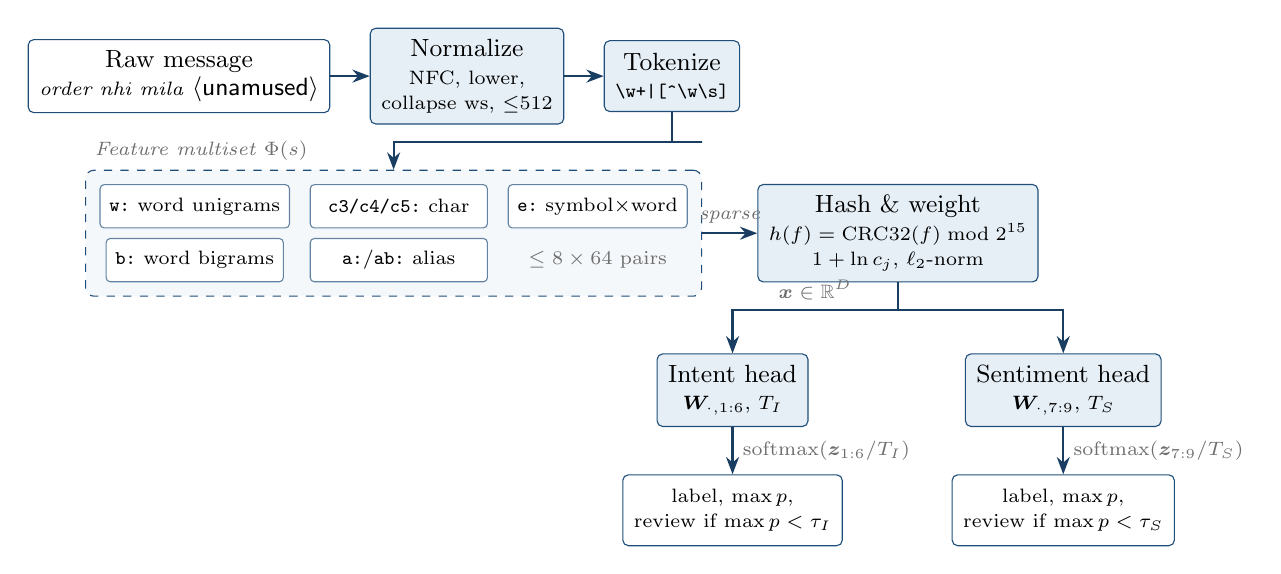
\begin{tikzpicture}[
  node distance=0.55cm and 0.5cm,
  box/.style={draw=accent,rounded corners=2pt,fill=accentlight!60,
              minimum height=0.9cm,align=center,font=\small,inner sep=4pt},
  ch/.style={draw=accent!70,rounded corners=1.5pt,fill=white,
             minimum width=2.25cm,minimum height=0.55cm,align=center,font=\scriptsize},
  arr/.style={-{Stealth[length=2.2mm]},thick,accent!80!black},
  lab/.style={font=\scriptsize\itshape,text=muted}]

  % input + normalizer
  \node[box,fill=white] (in) {Raw message\\[-1pt]\scriptsize\hi{order nhi mila} \emo{unamused}};
  \node[box,right=of in] (norm) {Normalize\\[-1pt]\scriptsize NFC, lower,\\[-2pt]\scriptsize collapse ws, $\le$512};
  \node[box,right=of norm] (tok) {Tokenize\\[-1pt]\scriptsize\verb!\w+|[^\w\s]!};

  % feature channels
  \node[ch,below=0.9cm of in,xshift=0.2cm]   (w)  {\texttt{w:}\ word unigrams};
  \node[ch,below=0.12cm of w]                (b)  {\texttt{b:}\ word bigrams};
  \node[ch,right=0.25cm of w]                (c)  {\texttt{c3/c4/c5:}\ char};
  \node[ch,below=0.12cm of c]                (a)  {\texttt{a:}/\texttt{ab:}\ alias};
  \node[ch,right=0.25cm of c]                (e)  {\texttt{e:}\ symbol$\times$word};
  \node[ch,below=0.12cm of e,draw=none,fill=none] (dummy) {\color{muted}\scriptsize$\le 8\times 64$ pairs};
  \begin{scope}[on background layer]
    \node[draw=accent,dashed,rounded corners=3pt,fill=accentlight!25,
          fit=(w)(b)(c)(a)(e)(dummy),inner sep=5pt,
          label={[lab,anchor=south west]north west:Feature multiset $\Phi(s)$}] (feat) {};
  \end{scope}

  % hashing + heads
  \node[box,right=0.7cm of feat] (hash) {Hash \& weight\\[-1pt]\scriptsize$h(f)=\mathrm{CRC32}(f)\bmod 2^{15}$\\[-2pt]\scriptsize$1+\ln c_j$, $\ell_2$-norm};
  \node[box,below=0.9cm of hash,xshift=-2.1cm] (hi) {Intent head\\[-1pt]\scriptsize$\W_{\cdot,1:6}$, $T_I$};
  \node[box,below=0.9cm of hash,xshift=2.1cm]  (hs) {Sentiment head\\[-1pt]\scriptsize$\W_{\cdot,7:9}$, $T_S$};
  \node[box,below=0.6cm of hi,fill=white] (oi) {\scriptsize label, $\max p$,\\[-2pt]\scriptsize review if $\max p<\tau_I$};
  \node[box,below=0.6cm of hs,fill=white] (os) {\scriptsize label, $\max p$,\\[-2pt]\scriptsize review if $\max p<\tau_S$};

  \draw[arr] (in) -- (norm);
  \draw[arr] (norm) -- (tok);
  \draw[arr] (tok.south) |- ($(feat.north east)+(0,0.35)$) -- ($(feat.north)+(0,0.35)$) -- (feat.north);
  \draw[arr] (feat) -- node[lab,above]{sparse} (hash);
  \draw[arr] (hash.south) -- ++(0,-0.35) -| node[lab,pos=0.25,above]{$\x\in\R^{D}$} (hi.north);
  \draw[arr] (hash.south) -- ++(0,-0.35) -| (hs.north);
  \draw[arr] (hi) -- node[lab,right]{$\softmax(\z_{1:6}/T_I)$} (oi);
  \draw[arr] (hs) -- node[lab,right]{$\softmax(\z_{7:9}/T_S)$} (os);
\end{tikzpicture}
\caption{Inference pipeline. A message is normalized, tokenized and expanded
into prefixed feature strings, which are hashed into a sparse,
$\ell_2$-normalized vector $\x$. Two linear softmax heads read disjoint columns
of one weight matrix and emit a label, a temperature-scaled confidence and a
review flag.}
\label{fig:arch}
\end{figure}

% ----------------------------------------------------------------------------
\subsection{Normalization and Tokenization}
\label{sec:norm}

The normalizer $\nu$ applies, in order: (i)~type check and rejection of inputs
longer than 512 code points; (ii)~Unicode NFC composition; (iii)~lower-casing;
(iv)~whitespace collapse; (v)~rejection of the empty string. Over-long input is
\emph{rejected} rather than truncated, because truncation can silently remove
a trailing negation or emoji---exactly the tokens that decide sentiment.
Lower-casing deliberately discards emphasis carried by capitalization
(\hi{SERIOUSLY}); this is a documented simplicity trade-off.

Tokens are extracted with the Unicode-aware pattern \verb!\w+|[^\w\s]!: a
maximal run of word characters in any script, or a \emph{single} non-space,
non-word code point. Consequently \hi{nahi!!!} yields
$\langle\hi{nahi},\,!,\,!,\,!\rangle$ and each emoji code point becomes its own
token. 

% ----------------------------------------------------------------------------
\subsection{Feature Channels}
\label{sec:features}

Given normalized string $\tilde s$ with tokens $t_{1:m}$, alias-expanded tokens
$u_{1:m'}$ and boundary-padded string $\hat s = {\texttt{\^{}}}\,\tilde s\,\texttt{\$}$, the
feature multiset is the union of the channels in \cref{tab:features}. Every
feature string carries a channel prefix, so a word \hi{kar} and a character
trigram \texttt{kar} hash independently.

\begin{table}[h]
\centering\small
\caption{Feature channels. \emph{Modes} lists the ablation configurations
that enable each channel (F = \lbl{full}, W = \lbl{word\_only}, C =
\lbl{char\_word}, S = \lbl{strip\_symbols}). Counts are distinct strings over
all 221 benchmark rows.}
\label{tab:features}
\begin{tabularx}{\linewidth}{@{}l X l r@{}}
\toprule
Prefix & Definition and purpose & Modes & Distinct \\
\midrule
\texttt{w:}  & $\{t_i\}$ --- unigrams; loanwords, emoji and punctuation as tokens & FWCS & 272 \\
\texttt{b:}  & $\{t_i|t_{i+1}\}$ --- adjacent pairs; short negation such as \hi{nahi|mila} & FWCS & 670 \\
\texttt{c3:}, \texttt{c4:}, \texttt{c5:} & all $n$-grams of $\hat s$, $n\in\{3,4,5\}$; spans word boundaries; shares substrings between \hi{delivery}/\hi{delivry} & F\,CS & 5{,}137 \\
\texttt{a:}  & $\{u_i\}$ --- tokens after the 20-entry alias map (\hi{nhi}$\to$\hi{nahi}, \hi{krdo}$\to$\hi{kar do}) & F\,\,\,\,S & 263 \\
\texttt{ab:} & $\{u_i|u_{i+1}\}$ --- alias bigrams & F\,\,\,\,S & 600 \\
\texttt{e:}  & $\{\sigma|\omega\}$ for the first $\le\!8$ unique Unicode-symbol tokens $\sigma$ and first $\le\!64$ unique alphanumeric tokens $\omega$; lets the model learn that \hi{badhiya} $\wedge$ \emo{unamused} differs from either alone & F\,\,\,\,S & 170 \\
\bottomrule
\end{tabularx}
\end{table}

Two design choices are especially important.

\emph{Additive, not destructive, aliasing.} The alias channel \emph{adds}
canonical-spelling features while keeping the raw tokens. Overwriting would
merge genuinely ambiguous forms (e.g.\ \hi{kaha} is both ``said'' and a
shorthand for \hi{kahan} ``where''); adding lets the learner weigh both.

\emph{Learned emoji semantics.} We do not assign any emoji a fixed polarity. The
interaction channel only creates the \emph{opportunity} to learn
context-dependent polarity; whether it is learned depends on data
(\cref{sec:emoji}). In \lbl{strip\_symbols} mode every code point in Unicode
general categories \texttt{S*} and \texttt{P*} is removed before tokenization,
so the \texttt{e:} channel is empty; this mode isolates the contribution of
symbols.

% ----------------------------------------------------------------------------
\subsection{Hashing and Vectorization}
\label{sec:hashing}

\begin{definition}[Hashed representation]
Let $D=2^{15}=32{,}768$ and $h(f) = \mathrm{CRC32}(\mathrm{UTF8}(f)) \bmod D$.
For multiset $\Phi(s)$ define counts $c_j=\lvert\{f\in\Phi(s): h(f)=j\}\rvert$ and
\begin{equation}
  \tilde x_j = \begin{cases} 1+\ln c_j & c_j>0\\ 0 & \text{otherwise}\end{cases},
  \qquad
  \x = \tilde\x \,/\, \max(\lVert\tilde\x\rVert_2,\,10^{-12}).
  \label{eq:vector}
\end{equation}
\end{definition}

CRC32 remains stable across processes and platforms, unlike Python's salted
\texttt{hash()}, so a saved model is portable. Sub-linear term frequency
($1+\ln c$) prevents a repeated token (\hi{!!!!!!}) from dominating, and
$\ell_2$ normalization makes scores comparable across message lengths---at the
cost of diluting a single decisive cue in a long message. $\x$ is stored
sparsely as sorted index/value arrays; messages in the benchmark activate
$F=130$ buckets on average (range 62--206).

% ----------------------------------------------------------------------------
\subsection{Two-Head Linear Model}
\label{sec:model}

The model uses a single matrix $\W\in\R^{D\times 9}$ and bias $\bb\in\R^{9}$ produce logits
$\z = \W^{\!\top}\x + \bb$. Columns $1{:}6$ form the intent head and $7{:}9$
the sentiment head:
\begin{equation}
  \p^{I} = \softmax\!\big(\z_{1:6}/T_I\big),\qquad
  \p^{S} = \softmax\!\big(\z_{7:9}/T_S\big).
  \label{eq:heads}
\end{equation}
For each task $k\in\{I,S\}$ the output is
$\hat y^{k}=\argmax_c p^{k}_c$, confidence $\max_c p^{k}_c$ and review flag
$\mathbb{1}[\max_c p^{k}_c<\tau_k]$. Because $\x$ is sparse, computing $\z$
costs $O(9F)$ rather than $O(9D)$.

\begin{proposition}[Decoupling]
\label{prop:decouple}
Both heads use the same input representation $\x$ but no trainable parameters.
The joint objective \eqref{eq:loss} is a sum of a term depending only on
$(\W_{\cdot,1:6},\bb_{1:6})$ and a term depending only on
$(\W_{\cdot,7:9},\bb_{7:9})$; weight decay is column-separable. Hence joint
training is exactly equivalent to training two independent classifiers with an
identical sample order.
\end{proposition}

\begin{remark}
The ``multi-task'' benefit of this architecture is therefore purely
computational (one feature extraction, one sparse row gather). Sharing
\emph{statistical strength} between intent and sentiment would require a
shared learned layer, which is out of scope for this baseline.
\end{remark}

\paragraph{Parameter budget.}
$|\theta| = 9D + 9 = 294{,}921$ learned scalars plus four fitted scalars
$(T_I,T_S,\tau_I,\tau_S)$---about $1{,}700\times$ below the 500M cap. Float32
weights occupy $1{,}179{,}684$ bytes; the compressed checkpoint is
$105{,}953$ bytes because only 4{,}556 of the 32{,}768 rows are non-zero after
training.

% ============================================================================
\section{Learning}
\label{sec:training}

\subsection{Objective}
Given a training set $\{(s_i,y^I_i,y^S_i)\}_{i=1}^{N}$ define class-balance
weights from training labels only,
$\alpha^{k}_{c}=N/\big(K_k\cdot\max(n^{k}_c,1)\big)$, where $n^{k}_c$ is the
count of class $c$ in task $k$. The per-sample objective (with $T=1$ during
training) is
\begin{equation}
  \mathcal{L}_i = \alpha^{I}_{y^I_i}\,\CE\!\big(\p^{I}(s_i),y^I_i\big)
                + \alpha^{S}_{y^S_i}\,\CE\!\big(\p^{S}(s_i),y^S_i\big).
  \label{eq:loss}
\end{equation}
On the training split, sentiment counts are 42/64/14, so a
\lbl{positive} example receives weight $120/(3\cdot14)=2.86$, versus $0.63$
for \lbl{neutral}.

\subsection{Optimization}
The softmax cross-entropy gradient with respect to the logits is
$\bm{g}=\alpha\,(\p-\bm{e}_y)$. Because $\x$ is sparse, only rows in
$\operatorname{supp}(\x)$ are touched. \Cref{alg:train} gives the procedure.

\begin{algorithm}[h]
\caption{Class-balanced sparse SGD with validation checkpointing}
\label{alg:train}
\small
\begin{algorithmic}[1]
\Require training rows, validation rows, epochs $E=55$, seed $42$
\State Precompute $(\mathcal{J}_i,\x_i)\gets$ \Call{Features}{$s_i$} for all training rows
\State $\W\gets\bm 0$, $\bb\gets\bm 0$, $\mathcal{L}^\star\gets\infty$
\For{$e=0,\dots,E-1$}
  \State $\eta_e\gets 0.6/(1+e/20)$
  \State $\W\gets 0.999\cdot\W$ \Comment{decoupled decay, once per epoch; bias not decayed}
  \For{$i$ in a seeded random permutation of $1..N$}
    \State $\z\gets\x_i^{\!\top}\W_{\mathcal{J}_i,\cdot}+\bb$
    \State $\bm g\gets[\softmax(\z_{1:6})-\bm e_{y^I_i}]\,\alpha^I_{y^I_i}\;\Vert\;[\softmax(\z_{7:9})-\bm e_{y^S_i}]\,\alpha^S_{y^S_i}$
    \State $\W_{\mathcal{J}_i,\cdot}\gets\W_{\mathcal{J}_i,\cdot}-\eta_e\,\x_i\bm g^{\!\top}$
    \State $\bb\gets\bb-0.1\,\eta_e\,\bm g$
  \EndFor
  \State $\mathcal{L}_{\text{val}}\gets$ mean \emph{unweighted} NLL over both heads on validation
  \If{$\mathcal{L}_{\text{val}}<\mathcal{L}^\star$} \State $\mathcal{L}^\star\gets\mathcal{L}_{\text{val}}$;\ store $(\W,\bb,e+1)$ \EndIf
\EndFor
\State \Return stored checkpoint
\end{algorithmic}
\end{algorithm}

\subsection{Calibration and Selective Prediction}
\label{sec:calibration}

After checkpoint selection, each head is calibrated independently on the
validation logits (\cref{alg:calib}).

\begin{algorithm}[h]
\caption{Per-head temperature scaling and review-threshold selection}
\label{alg:calib}
\small
\begin{algorithmic}[1]
\Require validation logits $\{\z_i\}$ and labels $\{y_i\}$ for one head
\State $\mathcal{G}\gets\{0.4\cdot 10^{k/29}: k=0,\dots,29\}$ \Comment{30 log-spaced values in $[0.4,4]$}
\State $T^\star\gets\argmin_{T\in\mathcal{G}}\frac1n\sum_i-\ln\softmax(\z_i/T)_{y_i}$
\State $q_i\gets\max_c\softmax(\z_i/T^\star)_c$, \ $r_i\gets\mathbb 1[\argmax=y_i]$
\State $\mathcal{C}\gets\big\{\tau\in\{0\}\cup\{q_i\}:\ |A_\tau|\ge5\ \wedge\ \overline{r}_{A_\tau}\ge0.90\big\}$, where $A_\tau=\{i:q_i\ge\tau\}$
\State $\tau^\star\gets$ element of $\mathcal{C}$ maximizing $|A_\tau|$, ties to the smallest $\tau$; \ $\tau^\star\gets1.01$ if $\mathcal{C}=\emptyset$
\State \Return $(T^\star,\tau^\star)$
\end{algorithmic}
\end{algorithm}

This rule maximizes \emph{coverage} while requiring an observed validation accuracy
of at least 90\% on accepted items, and falls back to ``review everything'' if
no threshold qualifies. Because there are only 43 validation rows from 18 groups, this is a
demonstration policy, not a statistical precision guarantee; the same split
is also used for checkpoint selection, so the estimate is optimistic.

\paragraph{Fitted values (full model).} $T_I=0.400$, $T_S=1.316$,
$\tau_I=0.000$ (accept all), $\tau_S=0.829$. Notably, $T_I$ lies on the
\emph{lower boundary} of the grid for all four configurations: the raw intent
logits are under-confident and the true NLL optimum may be sharper still.

% ============================================================================
\section{Benchmark Construction}
\label{sec:data}

\subsection{Seed Authoring}
We use no real customer data, scraped corpus, or teacher model. We authored
96 independent Hinglish seed messages, 16 per intent
(\cref{tab:seeds}). Sentiment is heavily skewed: positive affect exists
only within \lbl{feedback}, reflecting the realistic observation that
operational requests rarely express delight.

\begin{table}[h]
\centering\small
\caption{Seed composition by intent and base sentiment (negative / neutral / positive).}
\label{tab:seeds}
\begin{tabular}{@{}lcccccc|c@{}}
\toprule
 & \lbl{cancel} & \lbl{refund} & \lbl{track} & \lbl{not\_recv} & \lbl{damaged} & \lbl{feedback} & Total \\
\midrule
Neg / Neu / Pos & 4/12/0 & 5/11/0 & 4/12/0 & 6/10/0 & 7/9/0 & 4/4/8 & 30/58/8 \\
\bottomrule
\end{tabular}
\end{table}

\subsection{Group-First Splitting}
Each seed defines one \emph{group}. Within every (intent, base sentiment) stratum
with $n\ge3$ seeds, groups are shuffled with a fixed seed and assigned
$n_v=\max(1,\operatorname{round}(0.18n))$ to validation,
$n_t=\max(1,\operatorname{round}(0.22n))$ to test and the remainder to train;
strata with $n<3$ go entirely to train. Splitting happens \emph{before}
augmentation, and a validator rejects any group or lower-cased text that
appears in two splits.

\subsection{Augmentation}
Each seed can produce up to three deduplicated variants:
\begin{enumerate}
  \item the original;
  \item a \emph{shorthand} rewrite via a 10-entry map
        (\hi{nahi}$\to$\hi{nhi}, \hi{hai}$\to$\hi{h}, \hi{please}$\to$\hi{plz}, \dots);
  \item an \emph{orthographic} rewrite (\hi{order}$\to$\hi{ordr},
        \hi{delivery}$\to$\hi{delivry}, \hi{service}$\to$\hi{servis}).
\end{enumerate}
The augmentation process never adds or removes negation, emoji or punctuation. In
addition, each of the 8 positive \lbl{feedback} seeds spawns two contrast
forms: $s\,\emo{smile}$ labelled \lbl{positive} and $s\,\emo{unamused}$
labelled \lbl{negative}. This sarcasm convention is an annotation assumption
for these constructed pairs, not a universal emoji rule.

Because substitutions often do not apply, groups have 1, 2, 3, 6 or 9 rows
(22, 44, 26, 1 and 3 groups respectively), for $221$ rows in total
(\cref{tab:splits}).

\begin{table}[h]
\centering\small
\caption{Split statistics after augmentation.}
\label{tab:splits}
\begin{tabular}{@{}lrrc@{}}
\toprule
Split & Rows & Groups & Negative / Neutral / Positive \\
\midrule
Train      & 120 & 56 & 42 / 64 / 14 \\
Validation &  43 & 18 & 15 / 22 / \phantom{0}6 \\
Test       &  58 & 22 & 20 / 28 / 10 \\
\midrule
Audit (independent) & 24 & 24 & \phantom{0}7 / 15 / \phantom{0}2 \\
\bottomrule
\end{tabular}
\end{table}

\paragraph{Row-level vs.\ group-level sample size.} Rows within a group are
highly correlated. The effective sample size of the test split is closer to
its 22 groups than to its 58 rows, which motivates the cluster bootstrap in
\cref{sec:protocol}.

\subsection{Audit Set}
We also created a separate 24-example audit set (four per intent) was authored \emph{after} the
final model configuration was frozen and was never used for training,
calibration or tuning. It is still synthetic, single-author and partly
paraphrases the problem statement's own examples.

% ============================================================================
\section{Evaluation Protocol}
\label{sec:protocol}

\paragraph{Metrics.} Accuracy; per-class precision, recall and F1; macro-F1
(unweighted mean of class F1, the primary metric given class imbalance);
confusion matrices; \emph{coverage} (fraction with $\max p\ge\tau$) and
\emph{accepted accuracy}; expected calibration error (ECE, 10 equal-width bins).

\paragraph{Uncertainty.} For macro-F1, we report a 95\% percentile interval from a
\textbf{group-level cluster bootstrap} (5{,}000 resamples of the 22 test groups
with replacement, seed 0). Paired differences between configurations are
computed on the same resamples. For accuracies we additionally give Wilson
intervals, which treat rows as independent and are therefore optimistic.

\paragraph{Ablations.} We evaluate four configurations (\lbl{full}, \lbl{word\_only},
\lbl{char\_word}, \lbl{strip\_symbols}; \cref{tab:features}) are each
retrained and recalibrated from scratch with identical splits, seed and budget.

\paragraph{Stress test.} Only at evaluation time, a 14-entry map introduces
spellings \emph{never seen in training or augmentation}
(\hi{nahi}/\hi{nhi}$\to$\hi{nahii}, \hi{refund}$\to$\hi{refnd},
\hi{order}$\to$\hi{orrder}, \hi{hai}$\to$\hi{hey}, \dots) while preserving
negation, emoji and punctuation. This changes 89.7\% of the test messages. We report
macro-F1 on the perturbed set and \emph{prediction consistency}---agreement
with the model's own prediction on the clean text, which measures stability,
not correctness.

\paragraph{Emoji contrast pairs.} For every held-out pair
$(s,\ s\,\emo{unamused})$ labelled (\lbl{positive}, \lbl{negative}) we record
whether \emph{both} predictions are correct.

\paragraph{Honest status of the test split.} Test labels were never used for
checkpointing or calibration. However, preliminary test findings informed
development fixes, so we call it a \emph{development test}; the audit set is
the cleaner held-out estimate.

\paragraph{Latency.} Warm, serial, batch size 1; 80 warm-up and 600 timed
calls per workload; timing covers normalization, feature extraction, both
heads and JSON serialization, and excludes process start, model load, network
and queueing. Environment: Apple Silicon (arm64), macOS (Darwin 25.6.0),
Python 3.12.14, NumPy 2.3.5.

% ============================================================================
\section{Results}
\label{sec:results}

\subsection{Main Result and Ablations}

\begin{table}[t]
\centering\small
\caption{Development-test results for all configurations (58 rows, 22 groups).
Macro-F1 with 95\% group-bootstrap interval. Best clean score per column in bold.}
\label{tab:ablation}
\setlength{\tabcolsep}{4.5pt}
\begin{tabular}{@{}l cc cc cc c@{}}
\toprule
& \multicolumn{2}{c}{Intent} & \multicolumn{2}{c}{Sentiment} & \multicolumn{2}{c}{Stress macro-F1} & Train \\
\cmidrule(lr){2-3}\cmidrule(lr){4-5}\cmidrule(lr){6-7}
Config & Acc. & Macro-F1 [95\% CI] & Acc. & Macro-F1 [95\% CI] & Intent & Sent. & (s) \\
\midrule
\lbl{full}          &.810 &.820 [.568,.960] &.603 &.423 [.307,.526] &.717 &.449 & 0.57 \\
\lbl{word\_only}    &.586 &.607 [.405,.778] & \textbf{.638} & \textbf{.470} [.366,.573] &.454 & \textbf{.609} & 0.20 \\
\lbl{char\_word}    & \textbf{.845} & \textbf{.854} [.631,.955] &.603 &.429 [.321,.529] &.717 &.438 & 0.51 \\
\lbl{strip\_symbols}&.828 &.849 [.590, 1.00] &.483 &.327 [.207,.448] & \textbf{.736} &.400 & 0.56 \\
\bottomrule
\end{tabular}
\end{table}

\begin{figure}[t]
\centering
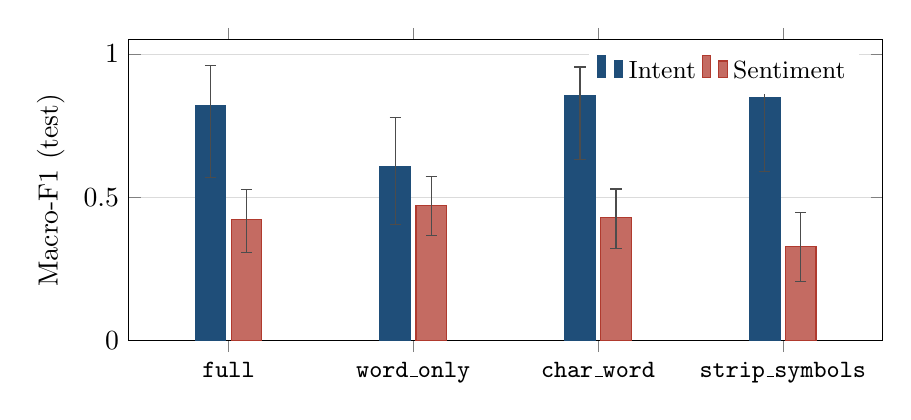
\begin{tikzpicture}
\begin{axis}[
  ybar=2pt, width=0.92\linewidth, height=5.4cm,
  ymin=0, ymax=1.05, ylabel={Macro-F1 (test)},
  symbolic x coords={full,word\_only,char\_word,strip\_symbols},
  xtick=data, xticklabel style={font=\small\ttfamily},
  enlarge x limits=0.18, bar width=11pt,
  legend style={font=\small,draw=none}, legend columns=2,
  legend pos=north east, ymajorgrids, grid style={muted!25},
  error bars/y dir=both, error bars/y explicit,
  error bars/error bar style={thin,black!70}]
\addplot[fill=accent,draw=accent] coordinates {
  (full,0.820) += (0,0.140) -= (0,0.252)
  (word\_only,0.607) += (0,0.171) -= (0,0.202)
  (char\_word,0.854) += (0,0.101) -= (0,0.223)
  (strip\_symbols,0.849) += (0,0.151) -= (0,0.259)};
\addplot[fill=warn!75,draw=warn] coordinates {
  (full,0.423) += (0,0.103) -= (0,0.116)
  (word\_only,0.470) += (0,0.103) -= (0,0.104)
  (char\_word,0.429) += (0,0.100) -= (0,0.108)
  (strip\_symbols,0.327) += (0,0.121) -= (0,0.120)};
\legend{Intent, Sentiment}
\end{axis}
\end{tikzpicture}
\caption{Ablation macro-F1 with 95\% group-bootstrap intervals. Intervals on
intent are wide because the test split contains only 22 paraphrase groups.}
\label{fig:ablation}
\end{figure}

\Cref{tab:ablation,fig:ablation} summarize the development test. Paired
bootstrap differences against \lbl{full} (\cref{tab:paired}) support three
conclusions and reject one tempting claim:

\begin{enumerate}
  \item \textbf{Character $n$-grams matter for intent.} Removing them
        (\lbl{word\_only}) lowers intent macro-F1 by $0.19$ (95\% CI
        $[-0.37,-0.03]$), and lowers stress-test intent F1 from
        $0.717$ to $0.454$.
  \item \textbf{Symbols carry sentiment signal.} Stripping symbols lowers
        sentiment macro-F1 by $0.09$ (CI $[-0.19,-0.01]$), and
        not one of the 5{,}000 resamples favoured \lbl{strip\_symbols}.
  \item \textbf{Sentiment is the bottleneck.} No configuration exceeds
        $0.47$ sentiment macro-F1.
  \item \textbf{Not supported: that alias and interaction channels help.}
        The simpler \lbl{char\_word} scores $+0.037$ above \lbl{full} on
        intent (CI $[-0.03,+0.12]$) and is statistically indistinguishable
        on sentiment. \lbl{word\_only} even has the best point estimate on
        sentiment. We retain \lbl{full} as the reference because it is the only
        configuration that \emph{can} represent emoji$\times$word context, not
        because it wins on this split.
\end{enumerate}

\begin{table}[h]
\centering\small
\caption{Paired group-bootstrap differences in test macro-F1 relative to \lbl{full}
(5{,}000 resamples). $P(\Delta>0)$ is the fraction of resamples favouring the alternative.}
\label{tab:paired}
\begin{tabular}{@{}l ccc ccc@{}}
\toprule
& \multicolumn{3}{c}{Intent} & \multicolumn{3}{c}{Sentiment}\\
\cmidrule(lr){2-4}\cmidrule(lr){5-7}
Alternative & $\overline\Delta$ & 95\% CI & $P(\Delta>0)$ & $\overline\Delta$ & 95\% CI & $P(\Delta>0)$\\
\midrule
\lbl{char\_word}     & $+0.037$ & $[-0.032,+0.115]$ & 0.81 & $+0.007$ & $[-0.031,+0.056]$ & 0.56\\
\lbl{word\_only}     & $\mathbf{-0.192}$ & $[-0.372,-0.030]$ & 0.01 & $+0.050$ & $[-0.061,+0.142]$ & 0.84\\
\lbl{strip\_symbols} & $+0.036$ & $[-0.030,+0.148]$ & 0.79 & $\mathbf{-0.094}$ & $[-0.192,-0.013]$ & 0.00\\
\bottomrule
\end{tabular}
\end{table}

\subsection{Per-Class Behaviour}

\begin{table}[h]
\centering\small
\caption{Row-normalized confusion matrices of the \lbl{full} model on the
development test (counts; shading $\propto$ row share). Rows are true labels.}
\label{tab:confusion}
\setlength{\tabcolsep}{5pt}
\begin{tabular}{@{}l cccccc c@{}}
\toprule
\multicolumn{8}{@{}l}{\textbf{(a) Intent}}\\
True $\backslash$ Pred & cancel & refund & track & not\_recv & damaged & feedback & F1 \\
\midrule
\lbl{cancel\_order} & \cm{44}{8} & 0 & \cm{16}{3} & 0 & 0 & 0 &.842 \\
\lbl{refund}        & 0 & \cm{60}{4} & 0 & 0 & 0 & 0 & 1.00 \\
\lbl{track\_order}  & 0 & 0 & \cm{60}{9} & 0 & 0 & 0 &.750 \\
\lbl{not\_received} & 0 & 0 & 0 & \cm{60}{8} & 0 & 0 &.889 \\
\lbl{damaged\_item} & 0 & 0 & 0 & \cm{17}{2} & \cm{34}{4} & \cm{9}{1} &.615 \\
\lbl{feedback}      & 0 & 0 & \cm{10}{3} & 0 & \cm{6}{2} & \cm{44}{14} &.824 \\
\midrule
\multicolumn{8}{@{}l}{\textbf{(b) Sentiment}}\\
True $\backslash$ Pred & negative & neutral & positive & & & & F1 \\
\midrule
\lbl{negative} & \cm{27}{9} & \cm{27}{9} & \cm{6}{2} & & & &.514 \\
\lbl{neutral}  & \cm{4}{2} & \cm{56}{26} & 0 & & & &.754 \\
\lbl{positive} & \cm{24}{4} & \cm{36}{6} & 0 & & & &.000 \\
\bottomrule
\end{tabular}
\end{table}

\Cref{tab:confusion} exposes two systematic failure modes. \textbf{Intent}
errors concentrate on semantically adjacent pairs:
\lbl{damaged\_item}$\to$\lbl{not\_received} (both involve ``delivered'') and
\lbl{cancel\_order}$\to$\lbl{track\_order} (``dispatch''). Four of 22 test
groups account for all 11 intent errors; 18 groups are fully correct.
\textbf{Sentiment} collapses toward the majority class: neutral recall is
0.93, but \emph{no} positive message is predicted positive. The positive
training signal comes from only 14 rows spanning a handful of praise words,
and held-out praise vocabulary (\hi{zabardast}, \hi{fantastic}) is unseen.

\subsection{Independent Audit}

\begin{table}[h]
\centering\small
\caption{Development test vs.\ independent audit (\lbl{full} model). Accuracy
with Wilson 95\% interval (row-independent, optimistic).}
\label{tab:audit}
\begin{tabular}{@{}l r cc cc@{}}
\toprule
& & \multicolumn{2}{c}{Intent} & \multicolumn{2}{c}{Sentiment}\\
\cmidrule(lr){3-4}\cmidrule(lr){5-6}
Set & $N$ & Acc. [95\% CI] & Macro-F1 & Acc. [95\% CI] & Macro-F1\\
\midrule
Development test & 58 &.810 [.691,.891] &.820 &.603 [.475,.719] &.423 \\
Audit            & 24 &.958 [.798,.993] &.958 &.917 [.742,.977] &.831 \\
\bottomrule
\end{tabular}
\end{table}

The audit scores are noticeably higher (\cref{tab:audit}). We interpret this as
\emph{sampling sensitivity}, not generalization: the audit contains only two
positive messages, draws on vocabulary close to the training seeds, and has
no augmentation variants. The two sets must not be pooled.

\subsection{Calibration and Review Coverage}

\begin{table}[h]
\centering\small
\caption{Calibration and selective prediction for the \lbl{full} model.
ECE uses 10 bins; ``mean conf.'' is the average top-class probability.}
\label{tab:calib}
\begin{tabular}{@{}ll cccc cc@{}}
\toprule
Head & Split & $T$ & ECE & Mean conf. & Accuracy & Coverage & Acc.\ on accepted\\
\midrule
Intent    & Validation & 0.400 & 0.102 & 0.852 & 0.907 & --- & --- \\
Intent    & Test ($T{=}1$)   & 1.000 & 0.333 & 0.534 & 0.810 & --- & --- \\
Intent    & Test       & 0.400 & 0.155 & 0.763 & 0.810 & 1.000 & 0.810 \\
\midrule
Sentiment & Validation & 1.316 & 0.134 & 0.715 & 0.605 & --- & --- \\
Sentiment & Test       & 1.316 & 0.139 & 0.657 & 0.603 & 0.138 & 1.000 \\
Audit: intent / sent.  & & & & & & 1.000 / 0.500 & 0.958 / 1.000 \\
\bottomrule
\end{tabular}
\end{table}

Temperature scaling reduces intent ECE by roughly half on test ($0.333\to0.155$) by sharpening
under-confident logits; for sentiment it barely changes ECE, and the head
remains \emph{over}-confident on validation. The review policy behaves very
differently per head (\cref{tab:calib}). For intent, $\tau_I=0$ accepts every
test item and the accepted accuracy (0.81) \emph{misses} the 0.90 validation
target---a direct consequence of fitting a threshold on 43 correlated rows.
For sentiment, $\tau_S=0.829$ accepts only 13.8\% of test messages, all of which
are correct; in practice the sentiment head functions as a
``flag-for-human'' signal rather than an autonomous classifier.

\subsection{Robustness to Unseen Misspellings}

\begin{table}[h]
\centering\small
\caption{Clean vs.\ stress-test performance (\lbl{full} model).}
\label{tab:stress}
\begin{tabular}{@{}l ccc@{}}
\toprule
Head & Clean macro-F1 & Stress macro-F1 & Prediction consistency \\
\midrule
Intent    & 0.820 & 0.717 \textcolor{warn}{($-0.103$)} & 79.3\% \\
Sentiment & 0.423 & 0.449 \textcolor{okgreen}{($+0.026$)} & 93.1\% \\
\bottomrule
\end{tabular}
\end{table}

Intent performance drops by about ten points and one in five predictions flips
(\cref{tab:stress}). Character $n$-grams provide partial tolerance---47.6\% of
the feature strings in an average test message never occur in training, yet
most predictions survive---but invariance is clearly not achieved. The small
sentiment \emph{gain} is within noise and reflects predictions that are
already near the majority class.

\subsection{Emoji Contrast Pairs}
\label{sec:emoji}

None of the four configurations solves \textbf{0 of 5} held-out
$(s,\ s\,\emo{unamused})$ pairs. These five pairs are spelling variants of only
two seed groups (\hi{support ekdum zabardast hai}, \hi{wah kya fantastic
service hai}), so this is two independent constructions, not five. The model
does predict \lbl{negative} for the \emo{unamused} form of the first seed, but
it also fails on the plain positive form, so the pair is not ``both correct.''
The interaction channel provides capacity for context-dependent emoji meaning;
eight training seeds are not enough to learn it.

\subsection{Efficiency}

\begin{table}[h]
\centering\small
\caption{Warm single-request latency (600 calls each) and serial throughput.}
\label{tab:latency}
\begin{tabular}{@{}l cccr@{}}
\toprule
Workload & p50 (ms) & p95 (ms) & p99 (ms) & Msg/s \\
\midrule
Test messages (mean 35 chars) & 0.155 & 0.218 & 0.227 & 6{,}218 \\
Synthetic, 32 code points     & 0.137 & 0.167 & 0.184 & 7{,}065 \\
Synthetic, 128 code points    & 0.327 & 0.376 & 0.425 & 2{,}982 \\
Synthetic, 512 code points    & 0.763 & 0.847 & 0.906 & 1{,}295 \\
\bottomrule
\end{tabular}
\end{table}

\begin{figure}[h]
\centering
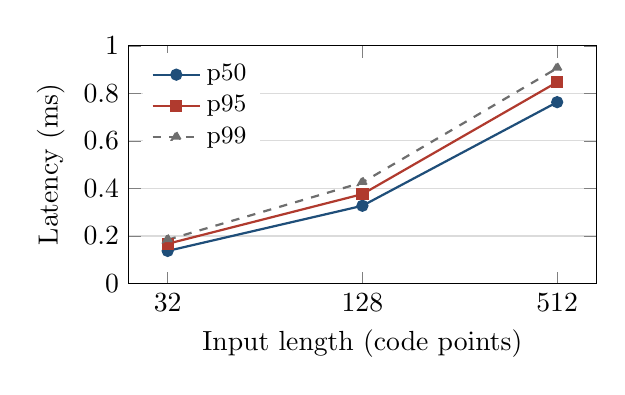
\begin{tikzpicture}
\begin{axis}[
  width=0.62\linewidth, height=4.6cm,
  xmode=log, log basis x=2, xtick={32,128,512},
  xticklabels={32,128,512}, xlabel={Input length (code points)},
  ylabel={Latency (ms)}, ymin=0, ymax=1.0,
  legend pos=north west, legend style={font=\small,draw=none},
  ymajorgrids, grid style={muted!25}, mark size=1.8pt]
\addplot[accent,thick,mark=*] coordinates {(32,0.137)(128,0.327)(512,0.763)};
\addplot[warn,thick,mark=square*] coordinates {(32,0.167)(128,0.376)(512,0.847)};
\addplot[muted,thick,dashed,mark=triangle*] coordinates {(32,0.184)(128,0.425)(512,0.906)};
\legend{p50, p95, p99}
\end{axis}
\end{tikzpicture}
\caption{Latency grows sub-linearly with length (16$\times$ longer input,
$\approx$5.6$\times$ slower). Even at the 512-code-point limit p99 is below 1\,ms.}
\label{fig:latency}
\end{figure}

Every workload meets the single-digit-millisecond target by roughly an order
of magnitude (\cref{tab:latency,fig:latency}). Training all four
configurations takes under two seconds in total. The fixed-length probes
repeat one sentence and thus produce fewer distinct features than varied text
of equal length; they are not a worst-case bound.

% ============================================================================
\section{Analysis}
\label{sec:analysis}

\subsection{Computational Complexity}
Let $L$ be the input length, $m$ the token count, $E\le8$ the selected symbol
tokens, $V\le64$ the selected word tokens and $F$ the number of distinct active
buckets. Feature extraction is $O(L+m+EV)$ string operations (three $n$-gram
lengths are a constant factor), sorting active indices is $O(F\log F)$, and
scoring is $O(F\cdot K)$ with $K=9$. Memory is $O(D\cdot K)$ for weights, and
$O(F)$ per request. The $EV\le512$ cross term bounds the worst case of the
interaction channel independently of $L$.

\subsection{Hash Collisions}
\label{sec:collisions}
Training data produce 4{,}921 distinct feature strings, which occupy 4{,}556
buckets---closely matching the $D\,[1-(1-1/D)^{n}]\approx4{,}569$ buckets
expected under uniform hashing. 14.4\% of training feature strings share a
bucket with at least one other string. Because hashing is unsigned, each
collision adds a biased rather than zero-mean perturbation. At this data scale
the effect is second-order compared with data scarcity; at production scale,
where the distinct-feature count would grow by orders of magnitude, a signed
hash or a larger $D$ (linear memory cost) would be
necessary.

\subsection{Qualitative Error Analysis}

\begin{table}[h]
\centering\small
\caption{Representative errors (\lbl{full} model) and their likely mechanism.}
\label{tab:errors}
\begin{tabularx}{\linewidth}{@{}p{4.9cm} p{2.9cm} X@{}}
\toprule
Message (set) & Gold $\to$ predicted & Interpretation \\
\midrule
\hi{cancel mat karna sirf order track karke batao} (audit) &
intent \lbl{track}$\to$\lbl{cancel} (conf.\ 0.996) &
\emph{Negation scope.} \hi{mat} negates \hi{cancel} two tokens later; bigrams
see \hi{cancel|mat} but cannot represent ``do \emph{not} cancel''. Highly
confident and wrong---the review flag does not fire. \\
\addlinespace
\hi{dispatch se pehle order rok do please} (test) &
intent \lbl{cancel}$\to$\lbl{track} (0.97) &
\emph{Lexical proxy.} \hi{dispatch} occurs in \lbl{track\_order} training
seeds; the paraphrase \hi{rok do} (``stop it'') for cancel is unseen. \\
\addlinespace
\hi{delivered item mein crack hai replace karna hai} (test) &
intent \lbl{damaged}$\to$\lbl{not\_recv} &
\emph{Keyword dominance.} \hi{delivered} is the strongest cue for
\lbl{not\_received}. \\
\addlinespace
\hi{bahut kharab experience tha} (test) &
sentiment \lbl{neg}$\to$\lbl{pos} &
\emph{Lexical co-occurrence.} \hi{bahut} and \hi{experience tha} occur in
positive \lbl{feedback} seeds (\hi{mast experience tha yaar}, \hi{service se
bahut khush hu}); the decisive \hi{kharab} is rare in training. \\
\addlinespace
\hi{bohot badhiya service} (audit) &
sentiment \lbl{pos}$\to$\lbl{neg} &
\emph{Contrast data dilutes praise words.} Every positive training seed also
appears with \emo{unamused} labelled negative, so praise words are observed
under both labels and carry little polarity alone; \hi{service} also occurs in
negative seeds (\hi{bekar service}). \\
\addlinespace
\hi{do hafte ho gaye refund nahi mila} (test) &
sentiment \lbl{neg}$\to$\lbl{neu} (flagged) &
\emph{Implicit affect.} Frustration expressed through elapsed time, not an
explicit sentiment word. Correctly routed to review. \\
\bottomrule
\end{tabularx}
\end{table}

\Cref{tab:errors} suggests that the dominant limitations are not tokenization
or speed, but (i)~a representation without compositional scope, and (ii)~a
training set too small to disentangle intent vocabulary, sentiment vocabulary
and emoji context.

% ============================================================================
% ============================================================================
\section{Version 1.1: Enriched Data and a Self-Attention Branch}
\label{sec:v11}

Version 1.1 acts on the first two items of the v1.0 future-work list. It adds
data first, then a representation upgrade, and re-runs the full protocol of
\cref{sec:protocol}. Everything in v1.0 that is not mentioned here is
unchanged: normalization, the six feature channels, hashing, class balancing,
checkpointing and calibration.

% ----------------------------------------------------------------------------
\subsection{Motivation}
The v1.0 analysis pointed to two separate causes of failure.
\begin{enumerate}
  \item \textbf{Label--intent confounding.} All 8 positive seeds belonged to
        \lbl{feedback} (\cref{tab:seeds}). The model could not separate
        ``positive'' from ``feedback vocabulary'', so positive recall on the
        test split was $0/10$ (\cref{tab:confusion}).
  \item \textbf{No word order beyond bigrams.} A bag of hashed features cannot
        represent which word a negator or an emoji modifies
        (\cref{tab:errors}). A layer in which every token can attend to every
        other token is the smallest change that gives the model this
        capacity.
\end{enumerate}

% ----------------------------------------------------------------------------
\subsection{Data Enrichment}
\label{sec:v11data}

We authored 117 new seeds, bringing the total to 213
(\cref{tab:v11seeds}). They were designed to break the confounding and to add
harder cases:
\begin{itemize}
  \item \textbf{Positive affect in every intent}, e.g.\ \hi{refund aa gaya
        account mein thank you so much} \emo{smile}, \hi{cancel ho gaya bina
        kisi hassle ke superb experience}, and resolved not-received cases
        (\hi{missing parcel neighbour ke paas mil gaya thank you});
  \item \textbf{explicit and implicit negatives} with varied vocabulary
        (\hi{loot}, \hi{jhoothe log}, \hi{fake otp}) and new emoji
        (\emo{huff});
  \item \textbf{negation minimal pairs} in \lbl{feedback}
        (\hi{service accha nahi laga} is \lbl{negative});
  \item \textbf{operational neutrals} with numbers and English terms
        (\hi{awb number se track kaise karu}, \hi{cod order ka refund kaise milega});
  \item \textbf{mixed messages} where praise and a request co-occur, labelled
        by the dominant expressed affect.
\end{itemize}
New seeds were checked against the audit set: no lower-cased audit text
appears in any split.

\begin{table}[h]
\centering\small
\caption{v1.1 seed composition by intent and base sentiment (negative / neutral / positive). Compare \cref{tab:seeds}.}
\label{tab:v11seeds}
\begin{tabular}{@{}lcccccc|c@{}}
\toprule
 & \lbl{cancel} & \lbl{refund} & \lbl{track} & \lbl{not\_recv} & \lbl{damaged} & \lbl{feedback} & Total \\
\midrule
Neg / Neu / Pos & 12/17/11 & 11/15/10 & 11/15/10 & 11/14/6 & 12/13/6 & 11/10/18 & 68/84/61 \\
\bottomrule
\end{tabular}
\end{table}

\paragraph{Augmentation.} Each form now yields up to five deduplicated variants
instead of three: the original, the shorthand rewrite, a \emph{respelling /
code-switch} rewrite from a 12-entry map (\hi{bahut}$\to$\hi{bohot},
\hi{parcel}$\to$\hi{parcl}, \hi{paise}$\to$\hi{money}, \hi{kab}$\to$\hi{when},
\dots), the composition of the two, and the original prefixed with one
tone-free opener chosen by the seeded generator (\hi{bhai}, \hi{hello team},
\hi{hi}, \hi{sir}, \hi{dekhiye}, \hi{ji}). The respelling map is disjoint from
the stress-test map, so the stress test still measures \emph{unseen} spellings.
Seven respellings were added to the alias channel (27 entries total).
Group-first splitting (\cref{sec:data}) is unchanged.

\begin{table}[h]
\centering\small
\caption{v1.1 split statistics after augmentation. Compare \cref{tab:splits}.}
\label{tab:v11splits}
\begin{tabular}{@{}lrrc@{}}
\toprule
Split & Rows & Groups & Negative / Neutral / Positive \\
\midrule
Train      & 536 & 130 & 187 / 181 / 168 \\
Validation & 158 &  39 & \phantom{0}50 / \phantom{0}58 / \phantom{0}50 \\
Test       & 190 &  44 & \phantom{0}64 / \phantom{0}65 / \phantom{0}61 \\
\midrule
Audit (unchanged) & 24 & 24 & \phantom{00}7 / \phantom{0}15 / \phantom{00}2 \\
\bottomrule
\end{tabular}
\end{table}

Sentiment is now close to balanced, so the class-balance weight of a positive
training row falls from $2.86$ to $536/(3\cdot168)=1.06$. The test split has
twice as many groups as in v1.0 (44 vs.\ 22), which narrows the bootstrap
intervals. Because the test split was \emph{regenerated}, v1.0 and v1.1 test
numbers are not paired and should be compared with caution.

% ----------------------------------------------------------------------------
\subsection{Self-Attention Branch}
\label{sec:v11att}

\paragraph{Token representation.} Let $t_{1:T}$ be the tokens of
$\nu(s)$ (after symbol stripping in \lbl{strip\_symbols} mode), truncated to
$T\le T_{\max}=128$ for this branch only. The linear branch still sees the
whole message. Each token $t_i$ is mapped to a set of hashed \emph{pieces}
$\mathcal{B}_i\subset\{0,\dots,B-1\}$, $B=2^{14}$: the word itself
(\texttt{tw:}), its alias (\texttt{ta:}, modes F and S) and its boundary-padded
character 3- and 4-grams (\texttt{tc3:}, \texttt{tc4:}, modes F, C and S).
With an embedding table $\bm E\in\R^{B\times d}$, $d=32$, and learned position
embeddings $\bm P\in\R^{T_{\max}\times d}$,
\begin{equation}
  \bm X_i = \frac{1}{|\mathcal{B}_i|}\sum_{j\in\mathcal{B}_i}\bm E_j + \bm P_i.
  \label{eq:v11embed}
\end{equation}
Averaging subword pieces, as in fastText, places
\hi{ordr} near \hi{order} before any training on the respelling.

\paragraph{Contextual layer and pooling.} One single-head scaled dot-product
self-attention layer with a residual connection and a $\tanh$ non-linearity,
followed by learned attention pooling:
\begin{align}
  \bm A &= \softmax_{\text{row}}\!\Big(\frac{(\bm X\bm W_Q)(\bm X\bm W_K)^{\!\top}}{\sqrt d}\Big) \in \R^{T\times T}, \label{eq:v11attn}\\
  \bm H &= \tanh\!\big(\bm X + \bm A\,\bm X\bm W_V\,\bm W_O\big) \in \R^{T\times d}, \label{eq:v11ctx}\\
  \bm\alpha &= \softmax(\bm H\bm u)\in\R^{T},\qquad
  \z^{\text{att}} = \Big(\textstyle\sum_{i}\alpha_i\bm H_i\Big)\bm W_{\text{out}}\in\R^{9}. \label{eq:v11pool}
\end{align}
Row $i$ of $\bm A$ controls which tokens update token $i$. For example, \hi{accha}
can take information from a following \hi{nahi}, and a trailing \emo{unamused}
can change the representation of the praise words before it. The pooling
weights $\bm\alpha$ show which contextualized tokens drive the decision, and
the app displays them.

\paragraph{Combination with v1.0.} The two branches are summed \emph{before}
the heads:
\begin{equation}
  \z = \underbrace{\W^{\!\top}\x + \bb}_{\text{v1.0 linear}} + \z^{\text{att}},\qquad
  \p^{I} = \softmax\!\big(\z_{1:6}/T_I\big),\quad
  \p^{S} = \softmax\!\big(\z_{7:9}/T_S\big).
  \label{eq:v11sum}
\end{equation}
The residual design keeps the v1.0 lexical strengths, while attention only
has to model what the linear branch gets wrong.

\begin{remark}
\Cref{prop:decouple} no longer holds. The heads now share $\bm E$, $\bm P$,
$\bm W_{Q,K,V,O}$ and $\bm u$, so the attention branch is a genuinely shared
multi-task layer. Only $\W_{\text{out}}$ and the linear parameters stay
column-separable.
\end{remark}

\begin{figure}[t]
\centering
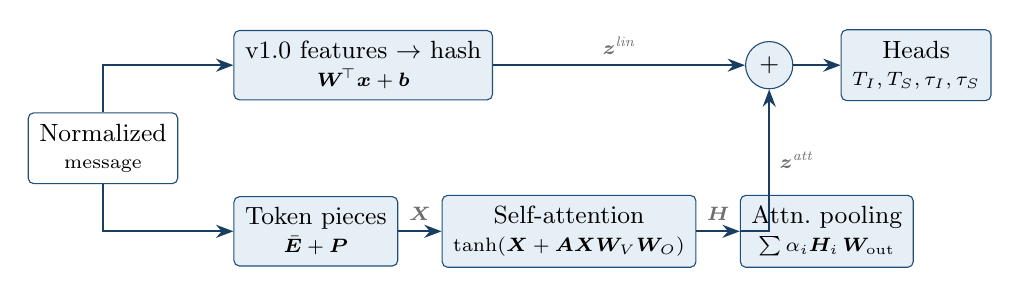
\begin{tikzpicture}[
  node distance=0.45cm and 0.55cm,
  box/.style={draw=accent,rounded corners=2pt,fill=accentlight!60,
              minimum height=0.85cm,align=center,font=\small,inner sep=4pt},
  arr/.style={-{Stealth[length=2.2mm]},thick,accent!80!black},
  lab/.style={font=\scriptsize\itshape,text=muted}]
  \node[box,fill=white] (in) {Normalized\\[-1pt]\scriptsize message};
  \node[box,above right=0.15cm and 0.7cm of in] (lin) {v1.0 features $\to$ hash\\[-1pt]\scriptsize$\W^{\!\top}\x+\bb$};
  \node[box,below right=0.15cm and 0.7cm of in] (emb) {Token pieces\\[-1pt]\scriptsize$\bar{\bm E}+\bm P$};
  \node[box,right=of emb] (att) {Self-attention\\[-1pt]\scriptsize$\tanh(\bm X+\bm A\bm X\bm W_V\bm W_O)$};
  \node[box,right=of att] (pool) {Attn.\ pooling\\[-1pt]\scriptsize$\sum\alpha_i\bm H_i\,\bm W_{\text{out}}$};
  \node[box,circle,inner sep=1pt,minimum height=0.6cm,right=3.2cm of lin] (plus) {$+$};
  \node[box,right=0.6cm of plus] (heads) {Heads\\[-1pt]\scriptsize$T_I,T_S,\tau_I,\tau_S$};
  \draw[arr] (in) |- (lin);
  \draw[arr] (in) |- (emb);
  \draw[arr] (emb) -- node[lab,above]{$\bm X$} (att);
  \draw[arr] (att) -- node[lab,above]{$\bm H$} (pool);
  \draw[arr] (lin) -- node[lab,above]{$\z^{\text{lin}}$} (plus);
  \draw[arr] (pool) -| node[lab,pos=0.75,right]{$\z^{\text{att}}$} (plus);
  \draw[arr] (plus) -- (heads);
\end{tikzpicture}
\caption{v1.1 architecture. The unchanged v1.0 linear branch (top) and the new
self-attention branch (bottom) produce 9 logits each. These are summed before
the temperature-scaled intent and sentiment heads.}
\label{fig:v11arch}
\end{figure}

\paragraph{Parameter budget.}
\begin{equation*}
  |\theta_{\text{att}}| = \underbrace{2^{14}\!\cdot\!32}_{\bm E=524{,}288}
  + \underbrace{128\!\cdot\!32}_{\bm P=4{,}096}
  + \underbrace{4\!\cdot\!32^2}_{\bm W_{Q,K,V,O}=4{,}096}
  + \underbrace{32}_{\bm u} + \underbrace{32\!\cdot\!9}_{\bm W_{\text{out}}=288}
  = 532{,}800,
\end{equation*}
so $|\theta| = 294{,}921 + 532{,}800 = 827{,}721$, still about $600\times$
below the 500M cap. The float32 arrays occupy 3{,}310{,}884 bytes. The
compressed checkpoint grows from 106\,KB to 2.22\,MB because $\bm E$ is dense
random-initialized, unlike the mostly zero $\W$.

\paragraph{Complexity.} The branch adds $O(\sum_i|\mathcal{B}_i|\,d + T^2 d + T d^2)$
per message. For typical messages ($T\approx 8$) this is dominated by the
embedding gather and the $d\times d$ projections, not the quadratic term.

% ----------------------------------------------------------------------------
\subsection{Training}
\label{sec:v11train}

Both branches are trained jointly on the class-balanced objective
\eqref{eq:loss}, using the combined logits \eqref{eq:v11sum}. The per-sample
logit gradient $\bm g$ of \cref{alg:train} is shared: the linear update is
unchanged, and $\bm g$ is also back-propagated through
\eqref{eq:v11pool}--\eqref{eq:v11embed}.

\paragraph{Gradients.} No autograd framework is used. With $\bm c=\sum_i\alpha_i\bm H_i$,
$\bm S=\bm Q\bm K^{\!\top}\!/\sqrt d$ and $\odot$ the element-wise product,
the backward pass is
\begin{align*}
  \nabla\bm W_{\text{out}} &= \bm c\,\bm g^{\!\top}, &
  \bm\delta_c &= \bm W_{\text{out}}\bm g,\\
  \delta\alpha_i &= \bm H_i\cdot\bm\delta_c, &
  \bm\delta_s &= \bm\alpha\odot\big(\bm{\delta\alpha} - (\bm\alpha^{\!\top}\bm{\delta\alpha})\bm 1\big),\\
  \nabla\bm u &= \bm H^{\!\top}\bm\delta_s, &
  \bm\delta_H &= \bm\alpha\,\bm\delta_c^{\!\top} + \bm\delta_s\bm u^{\!\top},\\
  \bm\Delta &= \bm\delta_H\odot(1-\bm H\odot\bm H), &
  \nabla\bm W_O &= (\bm A\bm V)^{\!\top}\bm\Delta,\\
  \bm\delta_A &= \bm\Delta\bm W_O^{\!\top}\bm V^{\!\top}, &
  \nabla\bm W_V &= \bm X^{\!\top}\bm A^{\!\top}\bm\Delta\bm W_O^{\!\top},\\
  \bm\delta_S &= \tfrac{1}{\sqrt d}\,\bm A\odot\big(\bm\delta_A - (\bm\delta_A\odot\bm A)\bm 1\bm 1^{\!\top}\big), &
  \nabla\bm W_Q &= \bm X^{\!\top}\bm\delta_S\bm K,\\
  \nabla\bm W_K &= \bm X^{\!\top}\bm\delta_S^{\!\top}\bm Q, &
  \bm V &= \bm X\bm W_V,
\end{align*}
and
\begin{equation*}
  \bm\delta_X=\bm\Delta+\bm\delta_S\bm K\bm W_Q^{\!\top}+\bm\delta_S^{\!\top}\bm Q\bm W_K^{\!\top}
  +\bm A^{\!\top}\bm\Delta\bm W_O^{\!\top}\bm W_V^{\!\top}.
\end{equation*}
Row $i$ of $\bm\delta_X$ goes to $\bm P_i$ and, divided by $|\mathcal{B}_i|$, to every
piece row $\bm E_j$, $j\in\mathcal{B}_i$. Every parameter group was checked against central
finite differences ($\epsilon=10^{-6}$, float64), with a maximum relative error
of $1.7\times10^{-5}$. The same check runs as a unit test.

\paragraph{Optimizers and regularization.} Dense attention parameters use Adam
($\beta=(0.9,0.999)$) and $\bm E$ uses sparse Adagrad, which updates only the
rows touched by a message. Both learning rates follow the v1.0 decay
$1/(1+e/20)$. Two regularizers proved necessary:
(i)~\textbf{token dropout}: each token is removed from the attention branch with
probability $0.2$ during training, so the branch cannot rely on a single
keyword; (ii)~\textbf{decoupled decay} of the dense attention matrices by
a factor $0.99$ once per epoch.

\paragraph{Hyper-parameter selection.} An untuned first run (Adam $3\!\times\!10^{-3}$,
Adagrad $0.05$, no regularization) overfit immediately: its validation-NLL
checkpoint was epoch~1. We then searched 11 settings and selected the one with
the \emph{lowest validation NLL} (\cref{tab:v11grid}). Test labels were not
used for this choice. However, the untuned run was scored once on the
development test, which remains a \emph{development} test as in v1.0.

\begin{table}[h]
\centering\small
\caption{Attention hyper-parameter search on the \lbl{full} configuration. NLL
is mean unweighted validation NLL at $T{=}1$ (before temperature scaling); the
linear-only v1.1 model scores $0.592$ on the same scale. Selected row in bold.}
\label{tab:v11grid}
\begin{tabular}{@{}cccc cc@{}}
\toprule
Adam lr & Adagrad lr ($\bm E$) & Token dropout & Dense decay & Best epoch & Val.\ NLL \\
\midrule
$10^{-3}$           & 0.02  & 0.0  & 0     &  2 & 0.659 \\
$3\times10^{-4}$    & 0.01  & 0.0  & 0     &  5 & 0.595 \\
$10^{-3}$           & 0.02  & 0.2  & 0     &  6 & 0.591 \\
$3\times10^{-4}$    & 0.01  & 0.2  & 0     & 18 & 0.558 \\
$10^{-3}$           & 0.02  & 0.2  & 0.02  & 18 & 0.557 \\
$10^{-4}$           & 0.005 & 0.1  & 0     & 18 & 0.550 \\
$3\times10^{-4}$    & 0.005 & 0.2  & 0.01  & 55 & 0.547 \\
$10^{-4}$           & 0.005 & 0.2  & 0     & 55 & 0.533 \\
$3\times10^{-4}$    & 0.01  & 0.3  & 0.01  & 52 & 0.526 \\
$2\times10^{-4}$    & 0.01  & 0.25 & 0.005 & 55 & 0.524 \\
$\mathbf{10^{-4}}$  & \textbf{0.01} & \textbf{0.2} & \textbf{0.01} & \textbf{55} & \textbf{0.516} \\
\bottomrule
\end{tabular}
\end{table}

The pattern is consistent: without token dropout, the attention branch
memorizes the 536 training rows within a few epochs and pulls the shared
logits away from the better-generalizing linear solution. With dropout and a
small learning rate, validation NLL improves over all 55 epochs. As in v1.0,
the checkpoint rule therefore never stops early. Training the \lbl{full}
configuration takes 12\,s on the same laptop, compared with 0.57\,s in v1.0.

% ----------------------------------------------------------------------------
\subsection{Results}
\label{sec:v11results}

\begin{table}[t]
\centering\small
\caption{v1.1 development-test results (190 rows, 44 groups). Macro-F1 with 95\%
group-bootstrap interval (5{,}000 resamples, seed 0). ``Linear only'' is the
\lbl{full} feature set trained on the enriched data \emph{without} the attention
branch. Best clean score per column in bold.}
\label{tab:v11main}
\setlength{\tabcolsep}{4pt}
\resizebox{\linewidth}{!}{%
\begin{tabular}{@{}l cc cc cc c@{}}
\toprule
& \multicolumn{2}{c}{Intent} & \multicolumn{2}{c}{Sentiment} & \multicolumn{2}{c}{Stress macro-F1} & Pos. \\
\cmidrule(lr){2-3}\cmidrule(lr){4-5}\cmidrule(lr){6-7}
Config & Acc. & Macro-F1 [95\% CI] & Acc. & Macro-F1 [95\% CI] & Intent & Sent. & recall \\
\midrule
Linear only (v1.1 data) &.863 &.860 [.720,.947] &.811 &.810 [.676,.911] &.797 & \textbf{.828} &.672 \\
\midrule
\lbl{full} + attention          & \textbf{.905} & \textbf{.901} [.782,.970] & \textbf{.847} & \textbf{.845} [.718,.944] & \textbf{.865} &.826 & \textbf{.721} \\
\lbl{word\_only} + attention    &.853 &.847 [.709,.929] &.826 &.827 [.714,.919] &.667 &.806 & \textbf{.721} \\
\lbl{char\_word} + attention    & \textbf{.905} & \textbf{.901} [.782,.970] &.832 &.831 [.704,.929] & \textbf{.865} &.816 & \textbf{.721} \\
\lbl{strip\_symbols} + attention&.884 &.888 [.757,.972] &.763 &.760 [.642,.860] &.853 &.795 &.639 \\
\midrule
\color{muted}v1.0 \lbl{full} (58-row test) & \color{muted}.810 & \color{muted}.820 [.568,.960] & \color{muted}.603 & \color{muted}.423 [.307,.526] & \color{muted}.717 & \color{muted}.449 & \color{muted}.000 \\
\bottomrule
\end{tabular}}
\end{table}

\begin{figure}[t]
\centering
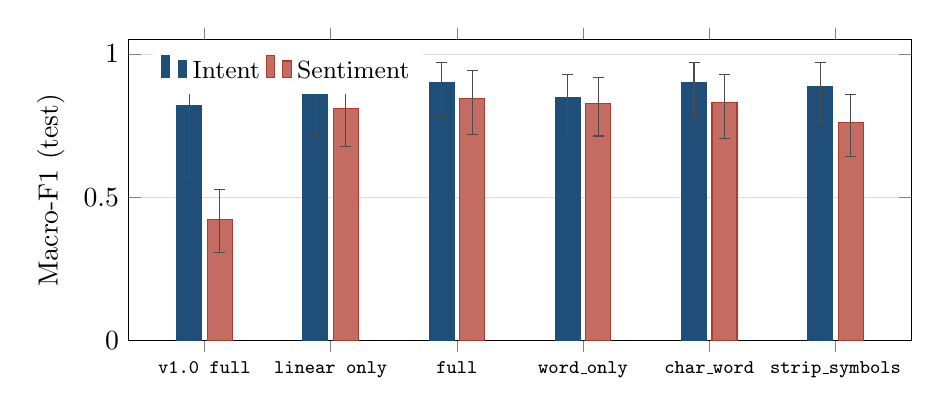
\begin{tikzpicture}
\begin{axis}[
  ybar=2pt, width=0.95\linewidth, height=5.4cm,
  ymin=0, ymax=1.05, ylabel={Macro-F1 (test)},
  symbolic x coords={v1.0 full,linear only,full,word\_only,char\_word,strip\_symbols},
  xtick=data, xticklabel style={font=\scriptsize\ttfamily},
  enlarge x limits=0.12, bar width=9pt,
  legend style={font=\small,draw=none}, legend columns=2,
  legend pos=north west, ymajorgrids, grid style={muted!25},
  error bars/y dir=both, error bars/y explicit,
  error bars/error bar style={thin,black!70}]
\addplot[fill=accent,draw=accent] coordinates {
  (v1.0 full,0.820) += (0,0.140) -= (0,0.252)
  (linear only,0.860) += (0,0.087) -= (0,0.140)
  (full,0.901) += (0,0.069) -= (0,0.119)
  (word\_only,0.847) += (0,0.082) -= (0,0.138)
  (char\_word,0.901) += (0,0.069) -= (0,0.119)
  (strip\_symbols,0.888) += (0,0.084) -= (0,0.131)};
\addplot[fill=warn!75,draw=warn] coordinates {
  (v1.0 full,0.423) += (0,0.103) -= (0,0.116)
  (linear only,0.810) += (0,0.101) -= (0,0.134)
  (full,0.845) += (0,0.099) -= (0,0.127)
  (word\_only,0.827) += (0,0.092) -= (0,0.113)
  (char\_word,0.831) += (0,0.098) -= (0,0.127)
  (strip\_symbols,0.760) += (0,0.100) -= (0,0.118)};
\legend{Intent, Sentiment}
\end{axis}
\end{tikzpicture}
\caption{Macro-F1 with 95\% group-bootstrap intervals. ``v1.0 full'' is measured
on the v1.0 test split; all other bars use the v1.1 test split. The largest
jump in sentiment (v1.0 $\to$ linear only) comes from the data. The step
from linear only to \lbl{full} comes from attention.}
\label{fig:v11bars}
\end{figure}

\begin{table}[h]
\centering\small
\caption{Paired group-bootstrap differences in v1.1 test macro-F1 relative to
\lbl{full}+attention (same 5{,}000 resamples). $P(\Delta>0)$ is the fraction of
resamples favouring the alternative.}
\label{tab:v11paired}
\begin{tabular}{@{}l ccc ccc@{}}
\toprule
& \multicolumn{3}{c}{Intent} & \multicolumn{3}{c}{Sentiment}\\
\cmidrule(lr){2-4}\cmidrule(lr){5-7}
Alternative & $\overline\Delta$ & 95\% CI & $P(\Delta>0)$ & $\overline\Delta$ & 95\% CI & $P(\Delta>0)$\\
\midrule
Linear only          & $-0.044$ & $[-0.101,+0.000]$ & 0.00 & $-0.036$ & $[-0.092,+0.002]$ & 0.04\\
\lbl{char\_word}     & $\phantom{+}0.000$ & $[\phantom{+}0.000,\phantom{+}0.000]$ & 0.00 & $-0.015$ & $[-0.043,+0.004]$ & 0.08\\
\lbl{word\_only}     & $\mathbf{-0.060}$ & $[-0.135,-0.007]$ & 0.00 & $-0.019$ & $[-0.108,+0.075]$ & 0.33\\
\lbl{strip\_symbols} & $-0.013$ & $[-0.056,+0.017]$ & 0.25 & $-0.086$ & $[-0.186,+0.019]$ & 0.05\\
\bottomrule
\end{tabular}
\end{table}

\Cref{tab:v11main,tab:v11paired,fig:v11bars} support four conclusions.
\begin{enumerate}
  \item \textbf{Data fixed the positive class.} Trained on the enriched data,
        even the linear-only model raises sentiment macro-F1 from $0.423$ to
        $0.810$ and positive recall from $0$ to $0.67$. This is the largest
        single improvement and confirms the v1.0 conclusion that data, not
        model size, was the bottleneck.
  \item \textbf{Attention adds a consistent, paired gain.} On identical data,
        adding the attention branch improves intent macro-F1 by $+0.044$ and
        sentiment by $+0.036$. None of the 5{,}000 resamples favours the
        linear-only model on intent, and 4\% favour it on sentiment. Both
        intervals touch zero at their upper end, so the gain is consistent
        but small relative to the data effect. Validation NLL after
        calibration improves from $0.543$ to $0.469$.
  \item \textbf{Attention mainly improves robustness to unseen spellings.}
        Stress-test intent macro-F1 rises from $0.797$ to $0.865$, and intent
        prediction consistency from $92.1\%$ to $97.4\%$. The subword-averaged
        embeddings \eqref{eq:v11embed} map \hi{orrder} and \hi{refnd} close
        to their clean forms.
  \item \textbf{Symbols still matter; alias/interaction channels still do not
        separate.} \lbl{strip\_symbols} is again the weakest on sentiment
        ($-0.086$, 95\% of resamples favour \lbl{full}). \lbl{char\_word}
        makes identical intent predictions to \lbl{full} and is within
        $0.015$ on sentiment, so the v1.0 finding in \cref{tab:paired} is
        unchanged.
\end{enumerate}

\begin{table}[h]
\centering\small
\caption{Row-normalized confusion matrices of the v1.1 \lbl{full} model on the
development test (counts; shading $\propto$ row share). Compare \cref{tab:confusion}.}
\label{tab:v11confusion}
\setlength{\tabcolsep}{5pt}
\begin{tabular}{@{}l cccccc c@{}}
\toprule
\multicolumn{8}{@{}l}{\textbf{(a) Intent}}\\
True $\backslash$ Pred & cancel & refund & track & not\_recv & damaged & feedback & F1 \\
\midrule
\lbl{cancel\_order} & \cm{60}{36} & 0 & 0 & 0 & 0 & 0 &.960 \\
\lbl{refund}        & \cm{9}{3} & \cm{51}{17} & 0 & 0 & 0 & 0 &.919 \\
\lbl{track\_order}  & 0 & 0 & \cm{58}{30} & \cm{2}{1} & 0 & 0 &.938 \\
\lbl{not\_received} & 0 & 0 & 0 & \cm{48}{21} & 0 & \cm{12}{5} &.875 \\
\lbl{damaged\_item} & 0 & 0 & 0 & 0 & \cm{43}{15} & \cm{17}{6} &.833 \\
\lbl{feedback}      & 0 & 0 & \cm{3}{3} & 0 & 0 & \cm{57}{53} &.883 \\
\midrule
\multicolumn{8}{@{}l}{\textbf{(b) Sentiment}}\\
True $\backslash$ Pred & negative & neutral & positive & & & & F1 \\
\midrule
\lbl{negative} & \cm{55}{59} & \cm{2}{2} & \cm{3}{3} & & & &.843 \\
\lbl{neutral}  & \cm{6}{7} & \cm{54}{58} & 0 & & & &.879 \\
\lbl{positive} & \cm{10}{10} & \cm{7}{7} & \cm{43}{44} & & & &.815 \\
\bottomrule
\end{tabular}
\end{table}

\paragraph{Per-class behaviour.} The collapse toward \lbl{neutral} seen in
v1.0 is gone: sentiment recall is $0.92$ / $0.89$ / $0.72$ and precision
$0.78$ / $0.87$ / $0.94$ for negative / neutral / positive
(\cref{tab:v11confusion}). The linear-only model reaches the same positive
precision but lower recall ($41$ vs.\ $44$ of $61$), and sends nine negatives
to neutral where attention sends two. Of the 17 remaining positive misses, 10 are predicted
\lbl{negative} and 7 \lbl{neutral}. Most are mixed messages in which praise
sits next to a complaint word or an unseen phrasing (\cref{tab:v11errors}). Intent errors
have moved: \lbl{cancel}$\leftrightarrow$\lbl{track} confusions are gone, and
most errors are now \lbl{not\_received}/\lbl{damaged\_item}$\to$\lbl{feedback}
for messages that open with praise of the support team.

\begin{table}[h]
\centering\small
\caption{Calibration, review coverage, stress test and emoji pairs (v1.1 \lbl{full}
vs.\ linear only, v1.1 test). ECE uses 10 bins.}
\label{tab:v11calib}
\begin{tabular}{@{}l cc cc@{}}
\toprule
& \multicolumn{2}{c}{Intent} & \multicolumn{2}{c}{Sentiment}\\
\cmidrule(lr){2-3}\cmidrule(lr){4-5}
Quantity & Linear only & \lbl{full}+att. & Linear only & \lbl{full}+att. \\
\midrule
Temperature $T$                 & 0.550 & 0.550 & 1.216 & 1.316 \\
Review threshold $\tau$          & 0.665 & 0.651 & 0.724 & 0.655 \\
ECE (test)                      & 0.043 & 0.082 & 0.102 & 0.106 \\
Mean confidence / accuracy      &.903 /.863 &.932 /.905 &.714 /.811 &.794 /.847 \\
Coverage / acc.\ on accepted    & --- &.953 /.906 & --- &.753 /.951 \\
Stress prediction consistency   & 92.1\% & 97.4\% & 90.0\% & 92.6\% \\
\midrule
Emoji contrast pairs both correct & \multicolumn{4}{l}{\footnotesize linear only 9/12 \quad \lbl{full} 9/12 \quad \lbl{char\_word} 9/12 \quad \lbl{word\_only} 7/12 \quad \lbl{strip\_symbols} 0/12} \\
\bottomrule
\end{tabular}
\end{table}

\paragraph{Calibration and review.} The selective-prediction policy is now
useful for both heads (\cref{tab:v11calib}). The sentiment head accepts
$75.3\%$ of test messages at $95.1\%$ accepted accuracy, compared with $13.8\%$
coverage in v1.0. The intent head accepts $95.3\%$ at $90.6\%$, meeting the
$0.90$ target that v1.0 missed. Attention makes the intent head slightly
\emph{over}-confident (ECE $0.043\to0.082$). Unlike v1.0 ($T_I=0.40$), neither temperature
is pinned at the grid boundary ($T_I=0.55$, $T_S=1.32$).

\paragraph{Emoji contrast pairs.} The held-out test now contains 12 pairs from
four independent seed groups. \lbl{full} solves 9 of 12, compared with 0 of 5
in v1.0. All three failures come from one group,
\hi{five star service keep it up} \emo{thumbs-up}, whose base form is
predicted negative. Removing symbols gives 0 of 12, as expected. The linear-only
model also solves 9 of 12, so on this metric the gain is attributable to the
data, not to attention.

\begin{table}[h]
\centering\small
\caption{Development test vs.\ independent audit for the v1.1 \lbl{full} model. Compare \cref{tab:audit}.}
\label{tab:v11audit}
\begin{tabular}{@{}l r cc cc@{}}
\toprule
& & \multicolumn{2}{c}{Intent} & \multicolumn{2}{c}{Sentiment}\\
\cmidrule(lr){3-4}\cmidrule(lr){5-6}
Set & $N$ & Accuracy & Macro-F1 & Accuracy & Macro-F1\\
\midrule
v1.1 development test & 190 &.905 &.901 &.847 &.845 \\
v1.1 audit            &  24 &.875 &.865 &.875 &.806 \\
\color{muted}v1.0 audit & \color{muted}24 & \color{muted}.958 & \color{muted}.958 & \color{muted}.917 & \color{muted}.831 \\
\bottomrule
\end{tabular}
\end{table}

\paragraph{Audit regression.} On the frozen 24-message audit, v1.1 makes 6
errors, while v1.0 made 3 (\cref{tab:v11audit}). One old error was fixed
(\hi{order cancellation chahiye bahut bekar experience hua} is now negative),
two remain (\hi{cancel mat karna \dots}, \hi{bohot badhiya service}) and four
are new. Two of the new errors are neutral negations predicted
\lbl{negative} (\hi{\dots kal ghar pe nahi hu}, \hi{normal sa experience tha
nothing special}). In the v1.1 training split, 74 of the 138 rows containing \hi{nahi}/\hi{nhi}
are negative (54\%, compared with 35\% of all rows). The model has partly
learned \hi{nahi}$\Rightarrow$\lbl{negative}. The other two are intent errors on short
messages (\hi{delivery phir late ghatiya service}$\to$\lbl{feedback},
\hi{parcel aaya par glass broken hai}$\to$\lbl{not\_received}). The audit is
tiny, with a Wilson interval on $21/24$ of $[0.69, 0.96]$, so this difference
is not statistically resolved. We did not tune on the audit, and we report
the regression as a warning that the new seeds introduced a spurious negation
cue.

\begin{table}[h]
\centering\small
\caption{v1.1 warm single-request latency (600 calls each; Apple M2, Python 3.14.7, NumPy 2.3.5). Compare \cref{tab:latency}.}
\label{tab:v11latency}
\begin{tabular}{@{}l cccr@{}}
\toprule
Workload & p50 (ms) & p95 (ms) & p99 (ms) & Msg/s \\
\midrule
Test messages                 & 0.307 & 0.427 & 0.478 & 3{,}165 \\
Synthetic, 32 code points     & 0.225 & 0.238 & 0.247 & 4{,}377 \\
Synthetic, 128 code points    & 0.571 & 0.584 & 0.613 & 1{,}763 \\
Synthetic, 512 code points    & 1.552 & 1.581 & 1.619 & 643 \\
\bottomrule
\end{tabular}
\end{table}

\paragraph{Efficiency.} The attention branch roughly doubles latency
(\cref{tab:v11latency}). The worst case, a 512-code-point message, is still
$1.6$\,ms at p99, well inside the single-digit-millisecond target. Latency
now grows faster with length ($6.9\times$ from 32 to 512 code points, compared
with $5.6\times$ in v1.0) because the attention branch processes every token.

% ----------------------------------------------------------------------------
\subsection{What Attention Looks At}
\label{sec:v11qual}

\begin{table}[h]
\centering\small
\caption{Attention-pooling weights $\bm\alpha$ of the v1.1 \lbl{full} model and its sentiment prediction.}
\label{tab:v11alpha}
\begin{tabularx}{\linewidth}{@{}X l@{}}
\toprule
Tokens with pooling weight & Sentiment \\
\midrule
\hi{accha}\,.50 \ \hi{laga}\,.50 & \lbl{positive} \\
\hi{accha}\,.30 \ \textbf{\hi{nahi}\,.40} \ \hi{laga}\,.30 & \lbl{negative} \\
\hi{bahut}\,.21 \ \hi{acchi}\,.21 \ \hi{service}\,.22 \ \hi{thank}\,.18 \ \hi{you}\,.18 & \lbl{positive} \\
\hi{bahut}\,.18 \ \hi{acchi}\,.19 \ \hi{service}\,.21 \ \hi{thank}\,.06 \ \hi{you}\,.10 \ \textbf{\emo{unamused}\,.25} & \lbl{negative} \\
\hi{cancel}\,.12 \ \hi{mat}\,.13 \ \hi{karna}\,.11 \ \hi{sirf}\,.16 \ \hi{order}\,.11 \ \hi{track}\,.11 \ \hi{karke}\,.14 \ \hi{batao}\,.12 & \lbl{neutral} (intent still \lbl{cancel}) \\
\bottomrule
\end{tabularx}
\end{table}

\Cref{tab:v11alpha} shows the intended behaviour on minimal pairs. Adding
\hi{nahi} or a trailing \emo{unamused} draws the largest pooling weight
\emph{and} shifts weight away from the praise tokens (\hi{thank} drops from
$0.18$ to $0.06$), and the sentiment flips. The negation-scope case from
v1.0 is \emph{not} solved. Pooling is almost uniform over
\hi{cancel mat karna sirf order track karke batao}, and the intent remains
\lbl{cancel\_order}. One attention layer trained on 536 rows has the capacity
to represent scope, but the data contain no ``\hi{X mat karna}, do Y''
examples from which to learn it. Pooling weights show what the classifier
reads. They are not a faithful causal explanation, and the linear branch
contributes independently.

\begin{table}[h]
\centering\small
\caption{Representative v1.1 errors on the development test (\lbl{full} model).}
\label{tab:v11errors}
\begin{tabularx}{\linewidth}{@{}p{5.0cm} p{3.0cm} X@{}}
\toprule
Message & Gold $\to$ predicted & Interpretation \\
\midrule
\hi{support team bahut acchi hai ek parcel receive nahi hua usme help karo} &
intent \lbl{not\_recv}$\to$\lbl{feedback} (0.86) &
\emph{Opening praise dominates.} The request comes after a long praise
clause, so both branches weight the \lbl{feedback} vocabulary. \\
\addlinespace
\hi{cancel ho gaya bina kisi hassle ke superb experience} &
sentiment \lbl{pos}$\to$\lbl{neg} (0.82) &
\emph{Negated negative.} \hi{bina \dots\ hassle} (``without hassle'') is
positive, but \hi{hassle} never occurs in training and \hi{bina} occurs only in
negative rows (\hi{bina parcel diye delivered kar diya}). This is the mirror
image of the negation-scope problem. \\
\addlinespace
\hi{bahut pareshan hu mera order cancel karo} &
sentiment \lbl{neg}$\to$\lbl{pos}/\lbl{neu} (0.37--0.44) &
\emph{Unseen affect word.} \hi{pareshan} (``troubled'') never occurs in
training, and \hi{bahut} often co-occurs with praise. The low confidence correctly triggers review. \\
\addlinespace
\hi{gate pe check kiya parcel nahi hai app says delivered} &
sentiment \lbl{neu}$\to$\lbl{neg} (0.71) &
\emph{Spurious \hi{nahi} cue}, the same mechanism as the audit regression. \\
\addlinespace
\hi{cancel ho gaya ab paise wapas chahiye} &
intent \lbl{refund}$\to$\lbl{cancel} (0.96) &
\emph{Keyword position.} The message opens with \hi{cancel}; the actual request
comes after \hi{ab}. \\
\bottomrule
\end{tabularx}
\end{table}

% ----------------------------------------------------------------------------
\subsection{Updated Scorecard}

\begin{table}[h]
\centering\small
\caption{Requirement status after v1.1. Compare \cref{tab:scorecard}.}
\label{tab:v11scorecard}
\begin{tabularx}{\linewidth}{@{}l l X@{}}
\toprule
Requirement & Status & Evidence \\
\midrule
$\le$500M parameters & \textcolor{okgreen}{\textbf{Met}} & 827{,}721 parameters (\cref{sec:v11att}). \\
Single-digit ms latency & \textcolor{okgreen}{\textbf{Met locally}} & p99 1.62\,ms at 512 code points (\cref{tab:v11latency}). \\
Spelling/shorthand robustness & \textcolor{okgreen}{\textbf{Improved}} & Unseen-misspelling intent F1 $0.865$ (v1.0: $0.717$); 97.4\% of intents unchanged. \\
Emoji and punctuation semantics & \textcolor{warn}{\textbf{Partial}} & Sarcasm pairs 9/12 (v1.0: 0/5), but from only four seed groups. \\
Positive sentiment & \textcolor{okgreen}{\textbf{Improved}} & Recall $0.72$, precision $0.94$ (v1.0: 0/10). \\
Negation scope & \textcolor{warn}{\textbf{Not met}} & \hi{cancel mat karna \dots} still wrong; new spurious \hi{nahi}$\Rightarrow$negative cue. \\
Reproducibility & \textcolor{okgreen}{\textbf{Met}} & Seeded, NumPy-only, 13 unit tests including a finite-difference gradient check. \\
\bottomrule
\end{tabularx}
\end{table}

\paragraph{Next steps after v1.1.} (i)~Add neutral seeds that contain
\hi{nahi} and positive seeds that contain negated negatives (\hi{koi problem
nahi}, \hi{bina hassle}) to remove the spurious negation cue.
(ii)~Add explicit negation-scope minimal pairs (\hi{cancel mat karna, track
karo}). (iii)~Report variance over several training seeds. The attention
branch adds randomness from initialization and token dropout, which a single
seed hides. (iv)~Refresh the audit with new, independently written messages,
because the current 24 examples are now partly out of distribution for the
enriched training set.

% ============================================================================
\section{Version 1.2: Distilling a Pretrained Hinglish Encoder into a Hashed-Piece Transformer}
\label{sec:v12}

Version 1.2 asks whether the remaining v1.1 failures are caused by missing
\emph{knowledge} or missing \emph{data}, and whether a small model can inherit
whatever fixes them. It fine-tunes a pretrained Hinglish encoder (the
\emph{teacher}) twice---once on the v1.1 training split alone and once with new
data---and distils the second teacher into an 11.88M-parameter \emph{student}
that keeps the v1.1 hashed pieces and the v1.0 linear branch and runs without
PyTorch. All numbers in this section come from \texttt{v12/results/*.json}.

% ----------------------------------------------------------------------------
\subsection{Motivation and Research Questions}
\label{sec:v12motivation}

The v1.1 error analysis (\cref{tab:v11errors}) and audit regression left four
documented failures: (a)~affect words unseen in training (\hi{pareshan},
\hi{bina \dots\ hassle}); (b)~a spurious \hi{nahi}$\Rightarrow$\lbl{negative}
cue; (c)~negation scope (\hi{cancel mat karna sirf order track karke batao});
and (d)~keyword-driven intent routing. The v1.1 next steps proposed targeted
data for (b) and (c), several seeds and a refreshed audit. v1.2 addresses the
first three and replaces the audit refresh with a separate hand-written
contrast set (\cref{sec:v12contrast}); the frozen 24-message audit is kept
unchanged for comparability.

\begin{enumerate}
  \item[\textbf{Q1}] Does pretrained Hinglish knowledge alone fix (a)--(d) Teacher trained on the v1.1 split only (\cref{sec:v12teacher1}).
  \item[\textbf{Q2}] Does more diverse, targeted data help beyond pretraining Same encoder and selection rule with new data (\cref{sec:v12teacher2}).
  \item[\textbf{Q3}] Does a student with at most 15M parameters and a p95 below 5\,ms (batch~1, laptop CPU, including hashing) keep the teacher's gains (\cref{sec:v12student,sec:v12results})
\end{enumerate}

\begin{figure}[t]
\centering
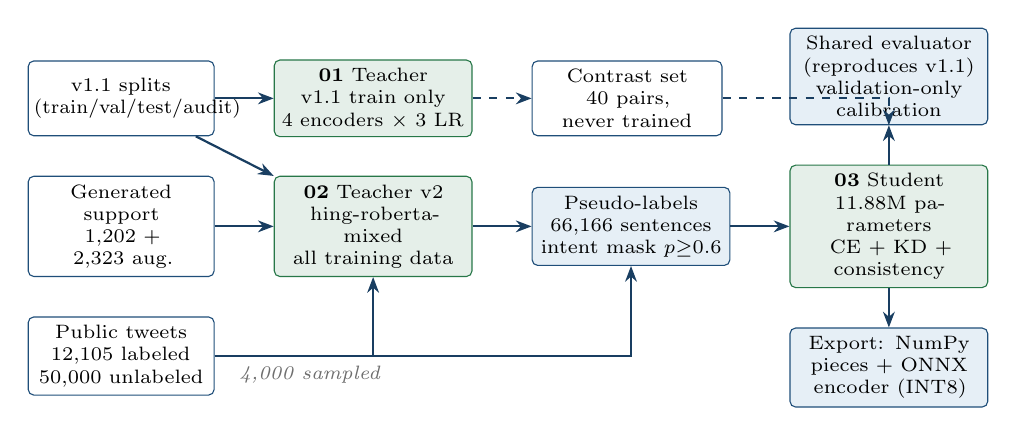
\begin{tikzpicture}[
  node distance=0.5cm and 0.45cm,
  box/.style={draw=accent,rounded corners=2pt,fill=accentlight!60,minimum height=0.95cm,align=center,font=\scriptsize,inner sep=3pt,text width=2.3cm},
  dat/.style={box,fill=white,text width=2.15cm},
  gpu/.style={box,fill=okgreen!12,draw=okgreen},
  arr/.style={-{Stealth[length=2mm]},thick,accent!80!black},
  lab/.style={font=\scriptsize\itshape,text=muted}]
  \node[dat] (v11) {v1.1 splits\\(train/val/test/audit)};
  \node[dat,below=of v11] (gen) {Generated support\\1{,}202 $+$ 2{,}323 aug.};
  \node[dat,below=of gen] (pub) {Public tweets\\12{,}105 labeled\\50{,}000 unlabeled};
  \node[gpu,right=0.75cm of v11] (t1) {\textbf{01} Teacher\\v1.1 train only\\4 encoders $\times$ 3 LR};
  \node[gpu,right=0.75cm of gen] (t2) {\textbf{02} Teacher v2\\hing-roberta-mixed\\all training data};
  \node[box,right=0.75cm of t2] (kd) {Pseudo-labels\\66{,}166 sentences\\intent mask $p{\ge}0.6$};
  \node[gpu,right=0.75cm of kd] (st) {\textbf{03} Student\\11.88M parameters\\CE $+$ KD $+$ consistency};
  \node[box,below=of st] (onnx) {Export: NumPy\\pieces $+$ ONNX\\encoder (INT8)};
  \node[box,above=of st] (eval) {Shared evaluator\\(reproduces v1.1)\\validation-only calibration};
  \node[dat,right=0.75cm of t1,text width=2.2cm] (con) {Contrast set\\40 pairs, never trained};
  \draw[arr] (v11) -- (t1);
  \draw[arr] (v11) -- (t2);
  \draw[arr] (gen) -- (t2);
  \draw[arr] (pub) -| node[lab,pos=0.3,below]{4{,}000 sampled} (t2);
  \draw[arr] (t2) -- (kd);
  \draw[arr] (kd) -- (st);
  \draw[arr] (pub.east) -| (kd.south);
  \draw[arr] (st) -- (onnx);
  \draw[arr] (st) -- (eval);
  \draw[arr,dashed] (t1) -- (con);
  \draw[arr,dashed] (con) -| (eval);
\end{tikzpicture}
\caption{v1.2 pipeline. Green boxes ran on a free Colab T4 as self-contained, automatically resuming notebooks (01: 38.4\,min; 02: 10.2\,min; 03: about 45\,min with one disconnect). Everything else ran on the laptop. Test, audit and contrast data are only scored.}
\label{fig:v12pipeline}
\end{figure}

% ----------------------------------------------------------------------------
\subsection{Protocol and Invariants}
\label{sec:v12protocol}

\begin{enumerate}
  \item \textbf{Exact v1.1 splits.} Train, validation, test and audit, with their group ids, are exported from the files whose SHA-256 digests are recorded in the v1.1 \texttt{results.json}; nothing is regenerated or reshuffled. A \texttt{test\_stress} copy applies the unchanged 14-entry stress map.
  \item \textbf{Validation only for choices.} Early stopping, model and learning-rate selection, temperature and review threshold use validation data only. Notebooks write test, audit and contrast logits; only the evaluator reads them.
  \item \textbf{All new data go to TRAIN, filtered.} A new message is dropped if its character-3-gram Jaccard similarity to any validation, test, audit or contrast message exceeds $0.6$:
  \begin{equation}
    J(a,b) = \frac{|G_3(a)\cap G_3(b)|}{|G_3(a)\cup G_3(b)|},\qquad G_3(s)=\{\text{3-grams of } \texttt{"\ "}\,\nu(s)\,\texttt{"\ "}\}.
    \label{eq:v12jaccard}
  \end{equation}
  An inverted index returns the exact intersection size and matches brute force on all 616 checked queries.
  \item \textbf{One evaluator.} A single evaluator scores every system from saved logits and reproduces every v1.1 test number in \cref{sec:v11results} exactly (macro-F1 and intervals, ECE, coverage, stress, emoji pairs, audit), so v1.1, teachers and students in this section are directly comparable.
  \item \textbf{Uncertainty.} As in v1.0 and v1.1: 5{,}000 resamples of the 44 test groups (seed 0); paired differences on identical resamples.
  \item \textbf{Hash parity.} The v1.1 hashing (\cref{eq:vector,eq:v11embed}) is copied into the training bundle and checked against 50 stored fixtures (indices exactly, values to $10^{-6}$) and a digest over all 1{,}148 exported rows. Results are identical under Python 3.10, 3.12, 3.13 (Colab) and 3.14, spanning Unicode databases 13.0--16.0. Every notebook reruns the fixture test before training.
\end{enumerate}

% ----------------------------------------------------------------------------
\subsection{Data}
\label{sec:v12data}

\subsubsection{Public Hinglish Data (Out of Domain)}
No public Hinglish customer-support \emph{intent} data was found. Public data
therefore contribute sentiment labels and unlabeled text for distillation only
(\cref{tab:v12public}). Cleaning repairs cp1252 mojibake, removes mentions,
URLs, \texttt{t.co} fragments and \texttt{RT}, keeps Latin-script letters only
(emoji and punctuation allowed), requires 3--60 words and at least two distinct
Romanized Hindi function words (English-ambiguous \hi{the, to, me, do, hi, ho,
na} excluded), and removes exact duplicates. \textbf{No public message was a
near-duplicate of a protected message.}
\begin{table}[h]
\centering
\small
\caption{Public sources after cleaning. The unlabeled pool is capped at 50{,}000 by seeded sampling.}
\label{tab:v12public}

\begin{tabularx}{\linewidth}{@{}X l r r@{}}
\toprule
Source & License & Raw & Kept \\
\midrule

SemEval-2020 Task 9 SentiMix, Hinglish
(re-upload \texttt{RTT1/SentiMix})
& research-use Twitter data
& 20{,}000
& 12{,}080 \\

Code-mixed tweets (\texttt{Abhishek4896/...})
& MIT
& 498
& 25 \\

PHINC (\texttt{LingoIITGN/PHINC})
& CC-BY-4.0
& 13{,}738
& 9{,}561 \\

L3Cube-HingLID (GitHub)
& CC-BY-NC-SA-4.0
& 44{,}455
& 42{,}543 \\

CMU Hinglish DoG (\texttt{festvox/cmu\_hinglish\_dog})
& CC-BY-SA-3.0
& 9{,}962
& 7{,}146 \\

\bottomrule
\end{tabularx}
\end{table}

Two candidates were rejected. A 100k ``code-mixed sentiment'' dataset turned out
to be machine-translated reviews mixing Devanagari, Bengali and English, not
Romanized Hinglish. The multi-GB L3Cube-HingCorpus file was not needed: HingLID
comes from the same L3Cube Twitter source. Twenty samples per source showed
political, cricket and movie content, frequent abuse and visible label noise in
SentiMix (for example, \hi{bht acha kiya \dots\ kr dena chahiye tha} labelled
neutral).

\subsubsection{Generated Support Data}
1{,}202 support messages in 591 paraphrase families (the plan was about 1{,}500)
were written by the LLM assistant in three batches. They cover all six intents
and three sentiments (\cref{tab:v12gen}); seven personas (student, elderly user,
shopkeeper, angry repeat customer, professional, homemaker, generic); 2--36
words (mean 11.3); 10.4\% with emoji; regional spellings (\hi{kaiku, apun,
kithe, kado}); formal Hindi (\hi{nivedan, nirast}) and heavy shorthand
(\hi{cncl, delvrd}). Rows are tagged by the phenomenon they target. One
near-duplicate was removed, and a lexical self-audit corrected two labels.

\begin{table}[h]
\centering\small
\caption{Generated data: label distribution (left) and targeted phenomena (right).}
\label{tab:v12gen}
\begin{tabular}{@{}lccc@{}}
\toprule
Intent & Neg & Neu & Pos \\
\midrule
\lbl{cancel\_order}  & 65 & 127 & 56 \\
\lbl{refund}         & 62 & 98 & 54 \\
\lbl{track\_order}   & 59 & 97 & 48 \\
\lbl{not\_received}  & 54 & 84 & 42 \\
\lbl{damaged\_item}  & 50 & 80 & 42 \\
\lbl{feedback}       & 61 & 57 & 66 \\
\midrule
Total (1{,}202)      & 351 & 543 & 308 \\
\bottomrule
\end{tabular}
\hspace{1.2em}
\begin{tabular}{@{}lr@{}}
\toprule
Tag & Rows \\
\midrule
negation scope & 97 \\
neutral with \hi{nahi} & 119 \\
negated negative & 99 \\
varied affect word & 151 \\
praise, then request & 82 \\
mixed intent (main request) & 66 \\
\bottomrule
\end{tabular}
\end{table}

\emph{Augmentation.} Each v1.1-train or generated row yields up to two
variants. The \emph{map} variant applies the v1.1 shorthand and respelling maps
per token with probability 0.6. The \emph{noise} variant applies vowel drop, a
QWERTY-neighbour swap, elongation or a transposition per editable token with
probability 0.3. Negators (\hi{nahi, mat, bina, koi, na, not}, \dots), emoji,
punctuation and numbers are never edited; token counts never change; and a
variant is rejected if it introduces a stress-map output (\hi{nahii, karr, hey,
orrder, refnd}, \dots), so the stress test stays unseen. This gives 2{,}323
variants (786 map, 1{,}537 noise), with 2 near-duplicates removed. A check over
17{,}680 noisy variants of every v1.1 text found no stress outputs and no edited
protected tokens.

\subsubsection{Diagnostic Contrast Set}
\label{sec:v12contrast}
Forty hand-written minimal pairs (80 messages) were written before any generated
data and are never used for training or selection: ten pairs each for
\emph{negation scope} (a negated action is not the request), \emph{neutral
nahi}, \emph{negated negative} and \emph{unseen affect}. The maximum Jaccard
similarity to any v1.1 message is 0.37. Each phenomenon is reported as the
fraction of messages with both labels correct and as the number of pairs whose
two members are both fully correct.

\paragraph{Overlap risk.} 18 of the 32 affect words in the contrast set
(\hi{pareshan, tang, dukhi, nirash, raahat, sukoon, chinta, prasann}, \dots)
enter training only through the generated data. Generated vocabulary also
raises coverage of the validation and test vocabulary from 0.687 and 0.701 to
0.949 and 0.944. For any model trained on generated data, \emph{unseen affect}
therefore measures learning from that data, not generalisation to new words.

% ----------------------------------------------------------------------------
\subsection{Teacher}
\label{sec:v12teacher}

\paragraph{Model.} A pretrained encoder $f_\phi$ produces subword states $\bm h_{1:n}$; masked mean pooling feeds two linear heads:
\begin{equation}
  \bar{\bm h} = \frac{\sum_{i} m_i \bm h_i}{\sum_i m_i},\qquad
  \z^{I} = \W_I\,\mathrm{Drop}(\bar{\bm h}) + \bb_I \in\R^{6},\qquad
  \z^{S} = \W_S\,\mathrm{Drop}(\bar{\bm h}) + \bb_S \in\R^{3}.
  \label{eq:v12teacher}
\end{equation}
The loss is the class-balanced cross-entropy of \cref{eq:loss}, with per-row head masks $\mu^k_i\in\{0,1\}$ (public sentiment rows have $\mu^I_i=0$):
\begin{equation}
  \mathcal{L}_{\text{T}} = \sum_{k\in\{I,S\}} \frac{1}{\sum_i\mu^k_i}\sum_i \mu^k_i\,\alpha^k_{y^k_i}\,\CE\big(\softmax(\z^k_i), y^k_i\big).
  \label{eq:v12teacherloss}
\end{equation}
Optimization uses AdamW (weight decay 0.01, none on biases or LayerNorm), linear warm-up then linear decay, gradient clipping at 1.0 and fp16 autocast with dynamic loss scaling. Early stopping uses the unweighted validation NLL of both heads, the v1.1 checkpoint criterion.

\begin{algorithm}[h]
\caption{Resumable fine-tuning run on a free GPU}
\label{alg:v12resume}
\small
\begin{algorithmic}[1]
\If{\texttt{status.json} marks the run done} \State \Return \Comment{``Run all'' again after a disconnect}\EndIf
\State load encoder; build optimizer, scheduler and loss scaler
\If{\texttt{last.pt} exists} \State restore weights (fp16), scheduler, RNG state, best NLL, patience counter, history \EndIf
\For{epoch $e$ from the resumed epoch to $E$}
  \State shuffle with a generator seeded by $1000\cdot\text{seed}+e$ \Comment{identical order after resuming}
  \State train; compute validation NLL; write \texttt{best.pt} if it improved
  \State write \texttt{last.pt} atomically (temporary file, then rename) to Google Drive
  \If{patience is exhausted} \textbf{break} \EndIf
\EndFor
\State load \texttt{best.pt}; write logits for every prediction file; mark done; delete checkpoints
\end{algorithmic}
\end{algorithm}

\subsubsection{Q1: Pretraining Only}
\label{sec:v12teacher1}
Four encoders---hing-roberta and hing-roberta-mixed, both
XLM-R base models; hing-bert; and
MuRIL---were each fine-tuned at three learning rates on
the 536-row v1.1 training split (batch 16, at most 12 epochs, patience 3).

\begin{table}[h]
\centering\small
\caption{Teacher runs on the v1.1 training split (Colab T4, 38.4\,min in total). Selection uses validation NLL only; test columns are shown for transparency and were not used.}
\label{tab:v12teacher1}
\setlength{\tabcolsep}{4pt}
\begin{tabular}{@{}l c c c c c c@{}}
\toprule
Run & Val.\ NLL & Test intent F1 & Test sent.\ F1 & Emoji pairs & Audit err. & Contrast both-correct \\
\midrule
hing-roberta, 2e-5          & 0.132 &.955 & 1.000 & 12/12 & 3 &.750 \\
hing-roberta, 3e-5          & 0.094 &.954 & 1.000 & 12/12 & 1 &.762 \\
hing-roberta, 5e-5          & 0.101 &.951 & 1.000 & 12/12 & 1 &.738 \\
hing-roberta-mixed, 2e-5    & 0.114 &.955 & 1.000 & 12/12 & 1 &.713 \\
hing-roberta-mixed, 3e-5    & 0.085 &.951 & 1.000 & 12/12 & 1 &.725 \\
\textbf{hing-roberta-mixed, 5e-5} & \textbf{0.080} & \textbf{.929} & \textbf{1.000} & \textbf{12/12} & \textbf{1} & \textbf{.738} \\
hing-bert, 2e-5             & 0.260 &.871 &.861 & 3/12 & 2 &.425 \\
hing-bert, 3e-5             & 0.253 &.903 &.896 & 9/12 & 2 &.475 \\
hing-bert, 5e-5             & 0.269 &.891 &.882 & 6/12 & 2 &.475 \\
muril-base-cased, 2e-5      & 1.296 &.863 &.791 & 0/12 & 3 &.500 \\
muril-base-cased, 3e-5      & 1.238 &.934 &.822 & 0/12 & 3 &.575 \\
muril-base-cased, 5e-5      & 1.143 &.923 &.828 & 0/12 & 4 &.475 \\
\bottomrule
\end{tabular}
\end{table}

\paragraph{Emoji visibility.} The BERT-vocabulary tokenizers (hing-bert and
MuRIL) map every emoji in all 261 emoji-bearing messages to \texttt{[UNK]}; the
XLM-R tokenizers keep them. This alone explains the 0--9/12 emoji-pair results.
The selected run has the lowest validation NLL even though it is not the best on
test intent, because selection never looks at test.

\paragraph{Verdict for Q1.} Pretraining fixes \emph{sentiment} on every set. Test sentiment macro-F1 is $1.000$, a paired $+0.159$ $[+0.056, +0.282]$ over v1.1; positive recall is $1.00$; average contrast sentiment accuracy is 0.96 versus 0.70; audit errors fall from 6 to 1. The 1.000 is a ceiling rather than leakage: validation sentiment accuracy is 0.943, no train and test groups overlap, and no test message has Jaccard similarity above 0.6 to any training message. \emph{Intent} is not resolved ($0.929$, paired $+0.032$ $[-0.061, +0.142]$). The teacher is also \emph{less} stable than v1.1 under unseen misspellings (consistency 92.6\% versus 97.4\%) and still routes \hi{cancel mat karna sirf order track karke batao} to \lbl{cancel\_order}.

\subsubsection{Q2: Teacher v2 (Pretraining and New Data)}
\label{sec:v12teacher2}
The same encoder and selection rule were trained on 8{,}061 rows: the v1.1
training split (536), generated messages (1{,}202), augmented variants (2{,}323)
and a fixed seeded sample of 4{,}000 public tweets with the intent loss masked
(batch 32, at most 6 epochs, patience 2, two learning rates; 10.2\,min on a T4).
The optional public-only pre-fine-tuning stage was skipped for time. Both runs
peaked at epoch 2, with validation NLL 0.0528 at 3e-5 and \textbf{0.0472} at
5e-5 (selected). The 3e-5 run scored higher on the contrast set (0.863 versus
0.825) and on stress intent (0.955 versus 0.933); it was not selected because
selection uses validation only.

\begin{table}[h]
\centering\small
\caption{Row-normalized test intent confusion matrices (counts; shading $\propto$ row share). Compare \cref{tab:v11confusion}.}
\label{tab:v12cm}
\setlength{\tabcolsep}{3.5pt}
\resizebox{\linewidth}{!}{%
\begin{tabular}{@{}l cccccc c cccccc c cccccc@{}}
\toprule
& \multicolumn{6}{c}{\textbf{v1.1}} && \multicolumn{6}{c}{\textbf{Teacher v2}} && \multicolumn{6}{c}{\textbf{Student $+$ KD (INT8)}}\\
\cmidrule(lr){2-7}\cmidrule(lr){9-14}\cmidrule(lr){16-21}
True & can & ref & trk & nrc & dmg & fb && can & ref & trk & nrc & dmg & fb && can & ref & trk & nrc & dmg & fb \\
\midrule
\lbl{cancel}   & \cm{60}{36} & 0 & 0 & 0 & 0 & 0 && \cm{60}{36} & 0 & 0 & 0 & 0 & 0 && \cm{58}{35} & 0 & \cm{2}{1} & 0 & 0 & 0 \\
\lbl{refund}   & \cm{9}{3} & \cm{51}{17} & 0 & 0 & 0 & 0 && \cm{3}{1} & \cm{57}{19} & 0 & 0 & 0 & 0 && \cm{9}{3} & \cm{51}{17} & 0 & 0 & 0 & 0 \\
\lbl{track}    & 0 & 0 & \cm{58}{30} & \cm{2}{1} & 0 & 0 && 0 & 0 & \cm{52}{27} & \cm{2}{1} & 0 & \cm{6}{3} && \cm{10}{5} & \cm{6}{3} & \cm{43}{22} & 0 & \cm{2}{1} & 0 \\
\lbl{not\_rcv} & 0 & 0 & 0 & \cm{48}{21} & 0 & \cm{12}{5} && 0 & 0 & 0 & \cm{60}{26} & 0 & 0 && 0 & 0 & 0 & \cm{60}{26} & 0 & 0 \\
\lbl{damaged}  & 0 & 0 & 0 & 0 & \cm{43}{15} & \cm{17}{6} && 0 & 0 & 0 & 0 & \cm{60}{21} & 0 && 0 & 0 & 0 & 0 & \cm{60}{21} & 0 \\
\lbl{feedback} & 0 & 0 & \cm{3}{3} & 0 & 0 & \cm{57}{53} && 0 & 0 & \cm{2}{2} & 0 & 0 & \cm{58}{54} && \cm{1}{1} & 0 & \cm{1}{1} & 0 & 0 & \cm{58}{54} \\
\bottomrule
\end{tabular}}
\end{table}

\paragraph{Verdict for Q2.} New data raise contrast negation-scope intent accuracy from 0.70 to 0.90 and fix the long-standing audit error. The \lbl{not\_received}$\to$\lbl{feedback} and \lbl{damaged}$\to$\lbl{feedback} confusions of v1.1 disappear (\cref{tab:v12cm}), stress intent F1 rises to 0.933, and 29 of 40 contrast pairs are solved. Against v1.1, intent is $0.966$ $[0.92, 0.99]$, a paired $+0.071$ $[-0.007, +0.172]$ that is borderline. The data effect over the Q1 teacher (same encoder) is \emph{not} resolved on 44 test groups: intent $+0.040$ $[-0.028, +0.121]$ with $P(\Delta>0)=0.85$, while sentiment is at the ceiling for both. The remaining errors are keyword-driven: \hi{otp nahi mila} and complaints about delays go to \lbl{not\_received}, and feedback about packing or delivery goes to operational intents.

\subsubsection{Pseudo-labels}
For every sentence $s$, teacher v2 provides logits $(\z^{I}_{\text{T}}, \z^{S}_{\text{T}})$. The KD masks are
\begin{equation}
  \kappa^I(s) = \mathbb{1}[s \in \text{support data}]\cdot\mathbb{1}\big[\max_c \softmax(\z^I_{\text{T}}(s))_c \ge 0.6\big],\qquad
  \kappa^S(s) = 1.
  \label{eq:v12mask}
\end{equation}

\begin{table}[h]
\centering\small
\caption{Pseudo-label statistics for the 66{,}166 distillation sentences.}
\label{tab:v12kd}
\begin{tabular}{@{}l r c c c@{}}
\toprule
KD set & Rows & Teacher = gold (intent) & Teacher = gold (sentiment) & Intent KD kept \\
\midrule
v1.1 train      & 536    & 1.000 & 1.000 & 1.000 \\
Generated       & 1{,}202 & 0.997 & 0.994 & 0.997 \\
Augmented       & 2{,}323 & 1.000 & 0.997 & 0.997 \\
Public labeled  & 12{,}105 & -- & 0.710 & 0 (masked) \\
Unlabeled pool  & 50{,}000 & -- & -- & 0 (masked) \\
\bottomrule
\end{tabular}
\end{table}

On support rows the teacher reproduces the gold labels it was trained on, so KD
there mainly transfers the \emph{shape} of the distribution. The new information
lies in the 62{,}105 public sentences. On the unlabeled pool the teacher predicts
22{,}902 neutral, 15{,}189 negative and 11{,}909 positive; its agreement with the
noisy SentiMix labels is 0.71.

% ----------------------------------------------------------------------------
\subsection{Student Architecture}
\label{sec:v12student}

\subsubsection{Input: the v1.1 Hashed Pieces}
Let $t_{1:T}$ be the tokens of $\nu(s)$ under the pattern \verb!\w+|[^\w\s]!, with $T\le T_{\max}=128$. Token $t_i$ yields the piece set
\begin{equation}
  \mathcal{B}_i = \Big\{h_B(\texttt{tw:}t_i),\; h_B(\texttt{ta:}\mathrm{alias}(t_i))\Big\}\cup\Big\{h_B(\texttt{tc}n\texttt{:}g): g \in \text{$n$-grams of } \texttt{<}t_i\texttt{>},\ n\in\{3,4\}\Big\},
  \label{eq:v12pieces}
\end{equation}
where $h_B(f)=\mathrm{CRC32}(\mathrm{UTF8}(f)) \bmod B$. The key strings are exactly those of v1.1 (\cref{eq:v11embed}); only the bucket count grows from $2^{14}$ to $B=2^{15}$ to reduce collisions from the 50{,}000-sentence pool.

\subsubsection{Encoder}
A pre-LayerNorm Transformer replaces the single v1.1 attention layer:
\begin{align}
  \bm X^{(0)}_i &= \frac{1}{|\mathcal{B}_i|}\sum_{j\in\mathcal{B}_i}\bm E_j + \bm P_i, && \bm E\in\R^{B\times d},\ \bm P\in\R^{T_{\max}\times d}, \label{eq:v12embed}\\
  \bm U^{(\ell)} &= \bm X^{(\ell-1)} + \mathrm{MHA}\big(\LN(\bm X^{(\ell-1)})\big), && \ell = 1,\dots,4, \\
  \bm X^{(\ell)} &= \bm U^{(\ell)} + \bm W_2\,\GELU\big(\bm W_1 \LN(\bm U^{(\ell)}) + \bm c_1\big) + \bm c_2, && \bm W_1\in\R^{1024\times d}, \\
  \mathrm{MHA}(\bm Y) &= \Big[\softmax\Big(\tfrac{\bm Q_h\bm K_h^{\!\top}}{\sqrt{d/4}} + \bm M\Big)\bm V_h\Big]_{h=1}^{4}\bm W_O, && [\bm Q,\bm K,\bm V] = \bm Y\bm W_{QKV}, \\
  \bm H &= \LN\big(\bm X^{(4)}\big),\quad \alpha_i = \softmax_i\big(\bm H_i\bm w_\alpha + b_\alpha + M_i\big),\quad \bm c = \textstyle\sum_i\alpha_i\bm H_i, \label{eq:v12pool}\\
  \z^{\text{enc}} &= \bm W_{\text{out}}\,\bm c + \bm b_{\text{out}} \in\R^{9}.
\end{align}
The width is $d=256$. Dropout 0.1 is applied to embeddings, attention weights and both residual branches. $\bm M$ adds $-10^4$ on padded keys, and attention and pooling softmaxes are computed in float32 under fp16 autocast. The token embedding is an \texttt{EmbeddingBag} in mean mode, the batched form of \cref{eq:v11embed}.

\subsubsection{Residual Hashed Linear Branch}
As in v1.1 (\cref{eq:v11sum}), the v1.0 linear model over the feature channels of \cref{tab:features} is kept and its logits are added before the heads:
\begin{equation}
  \z = \underbrace{\z^{\text{enc}}}_{\text{contextual}} + \underbrace{\W_L^{\!\top}\x + \bb_L}_{\text{lexical (v1.0)}},\qquad
  \p^{I}=\softmax(\z_{1:6}/T_I),\quad \p^{S}=\softmax(\z_{7:9}/T_S),
  \label{eq:v12sum}
\end{equation}
where $\W_L$ is initialised to zero (as in v1.0) and implemented as a sum-mode \texttt{EmbeddingBag} with per-sample weights $\x$.

\begin{figure}[t]
\centering
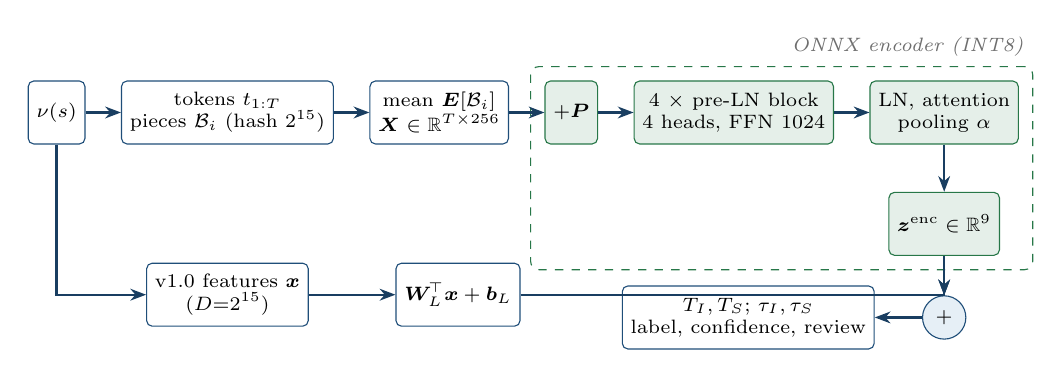
\begin{tikzpicture}[
  node distance=0.35cm and 0.45cm,
  box/.style={draw=accent,rounded corners=2pt,fill=accentlight!60,minimum height=0.8cm,align=center,font=\scriptsize,inner sep=3pt},
  np/.style={box,fill=white},
  onnx/.style={box,fill=okgreen!12,draw=okgreen},
  arr/.style={-{Stealth[length=2mm]},thick,accent!80!black},
  lab/.style={font=\scriptsize\itshape,text=muted}]
  \node[np] (txt) {$\nu(s)$};
  \node[np,right=of txt] (tok) {tokens $t_{1:T}$\\pieces $\mathcal{B}_i$ (hash $2^{15}$)};
  \node[np,right=of tok] (emb) {mean $\bm E[\mathcal{B}_i]$\\$\bm X\in\R^{T\times256}$};
  \node[onnx,right=of emb] (pos) {$+\bm P$};
  \node[onnx,right=of pos] (blk) {4 $\times$ pre-LN block\\4 heads, FFN 1024};
  \node[onnx,right=of blk] (pool) {LN, attention\\pooling $\alpha$};
  \node[onnx,below=0.6cm of pool] (head) {$\z^{\text{enc}}\in\R^9$};
  \node[np,below=1.5cm of tok] (feat) {v1.0 features $\x$\\($D{=}2^{15}$)};
  \node[np,right=1.1cm of feat] (lin) {$\W_L^{\!\top}\x+\bb_L$};
  \node[box,circle,inner sep=1pt,minimum height=0.55cm,below=0.5cm of head] (plus) {$+$};
  \node[np,left=0.6cm of plus] (cal) {$T_I,T_S$; $\tau_I,\tau_S$\\label, confidence, review};
  \draw[arr] (txt) -- (tok);
  \draw[arr] (tok) -- (emb);
  \draw[arr] (emb) -- (pos);
  \draw[arr] (pos) -- (blk);
  \draw[arr] (blk) -- (pool);
  \draw[arr] (pool) -- (head);
  \draw[arr] (txt) |- (feat);
  \draw[arr] (feat) -- (lin);
  \draw[arr] (lin) -| (plus);
  \draw[arr] (head) -- (plus);
  \draw[arr] (plus) -- (cal);
  \begin{scope}[on background layer]
    \node[draw=okgreen,dashed,rounded corners=3pt,fit=(pos)(blk)(pool)(head),inner sep=5pt,
          label={[lab,anchor=south east]north east:ONNX encoder (INT8)}] {};
  \end{scope}
\end{tikzpicture}
\caption{Student at inference. White boxes run in NumPy (hashing, embedding mean, linear branch, calibration); the green region is the exported ONNX encoder. Compare the v1.1 architecture in \cref{fig:v11arch}.}
\label{fig:v12student}
\end{figure}

\begin{table}[h]
\centering\small
\caption{Parameter breakdown compared with v1.1 (\cref{sec:v11att}).}
\label{tab:v12params}
\begin{tabular}{@{}l r r@{}}
\toprule
Component & v1.1 & v1.2 student \\
\midrule
Piece embeddings & $2^{14}\times32 = 524{,}288$ & $2^{15}\times256 = 8{,}388{,}608$ \\
Positions & $128\times32 = 4{,}096$ & $128\times256 = 32{,}768$ \\
Contextual layers & 1 single-head attention: 4{,}096 & 4 pre-LN blocks: 3{,}159{,}040 \\
Pooling and output & $32 + 288 = 320$ & 3{,}082 \\
Hashed linear branch & 294{,}921 & 294{,}921 \\
\midrule
\textbf{Total} & \textbf{827{,}721} & \textbf{11{,}878{,}419} \\
Without the linear branch & 532{,}800 & 11{,}583{,}498 \\
\bottomrule
\end{tabular}
\end{table}

\begin{table}[h]
\centering\small
\caption{Architectural differences between the v1.1 attention branch and the v1.2 student.}
\label{tab:v12diff}
\begin{tabularx}{\linewidth}{@{}l X X@{}}
\toprule
& v1.1 attention branch & v1.2 student \\
\midrule
Token representation & mean of hashed pieces, $B=2^{14}$, $d=32$ & same pieces, $B=2^{15}$, $d=256$ \\
Context & 1 layer, 1 head, residual $\tanh$, no FFN, no LayerNorm & 4 pre-LN layers, 4 heads, GELU FFN 1024 \\
Pooling & $\softmax(\bm H\bm u)$ & $\softmax(\bm H\bm w_\alpha + b_\alpha)$ with padding mask \\
Lexical branch & v1.0 linear, logits added & identical \\
Training signal & gold labels only & gold labels, teacher soft labels and consistency \\
Optimizer & per-example Adam and sparse Adagrad (NumPy, hand-derived gradients) & AdamW, cosine schedule, fp16, batch 64 (PyTorch) \\
Runtime & NumPy & NumPy and ONNX Runtime (INT8) \\
\bottomrule
\end{tabularx}
\end{table}

\subsubsection{Objective}
With student logits $\z$, teacher logits $\z_{\text{T}}$, gold-label masks $\mu$, KD masks $\kappa$ (\cref{eq:v12mask}) and a meaning-preserving noisy copy $\tilde s$, following knowledge distillation:
\begin{align}
  \mathcal{L}_{\text{CE}} &= \sum_{k} \frac{1}{\sum_i\mu^k_i}\sum_i \mu^k_i\,\alpha^k_{y^k_i}\,\CE\big(\softmax(\z^k_i), y^k_i\big), \\
  \mathcal{L}_{\text{KD}} &= \sum_{k} \frac{1}{\sum_i\kappa^k_i}\sum_i \kappa^k_i\; \tau^2\,\KL\Big(\softmax(\z^k_{\text{T},i}/\tau)\,\Big\|\,\softmax(\z^k_i/\tau)\Big),\qquad \tau = 2, \\
  \mathcal{L}_{\text{cons}} &= \frac{1}{N}\sum_i\sum_k \KL\Big(\mathrm{sg}\big[\softmax(\z^k(s_i))\big]\,\Big\|\,\softmax(\z^k(\tilde s_i))\Big), \\
  \mathcal{L}_{\text{S}} &= \mathcal{L}_{\text{CE}} + \lambda_{\text{KD}}\,\mathcal{L}_{\text{KD}} + \lambda_{\text{cons}}\,\mathcal{L}_{\text{cons}},\qquad \lambda_{\text{KD}}=1,\ \lambda_{\text{cons}}=0.1.
  \label{eq:v12loss}
\end{align}
Here $\mathrm{sg}$ is stop-gradient. The noisy copy $\tilde s$ uses only the character noise of \cref{sec:v12data}, so consistency is never imposed across meaning-changing edits (negation, emoji).

\paragraph{Training.} Every epoch uses all 4{,}061 support rows plus 4{,}000 public labeled tweets and 8{,}000 pool sentences, both re-sampled each epoch with a generator seeded by $1000\cdot\text{seed}+e$ (16{,}061 rows, 251 steps at batch 64, about 42\,s per epoch on a T4). Token dropout removes whole tokens with probability 0.15, always keeping at least one. Optimization uses AdamW (learning rate $5\times10^{-4}$, weight decay 0.01 except on embeddings, norms and biases), 5\% warm-up then cosine decay, clipping at 1.0 and fp16 autocast. Early stopping uses validation NLL (patience 5, at most 30 epochs). The full optimizer, scheduler, scaler and RNG state is checkpointed every epoch. Temperatures and review thresholds are fitted on validation with the v1.0 algorithm (\cref{alg:calib}).

\paragraph{Variants.} In order: student $+$ KD (seed 42, the pre-specified primary model); student without KD on identical labeled data (pool rows drop out automatically); student $+$ KD without the linear branch; and student $+$ KD with seeds 43 and 44. All five finished, with one Colab disconnect resumed automatically.

\begin{figure}[t]
\centering
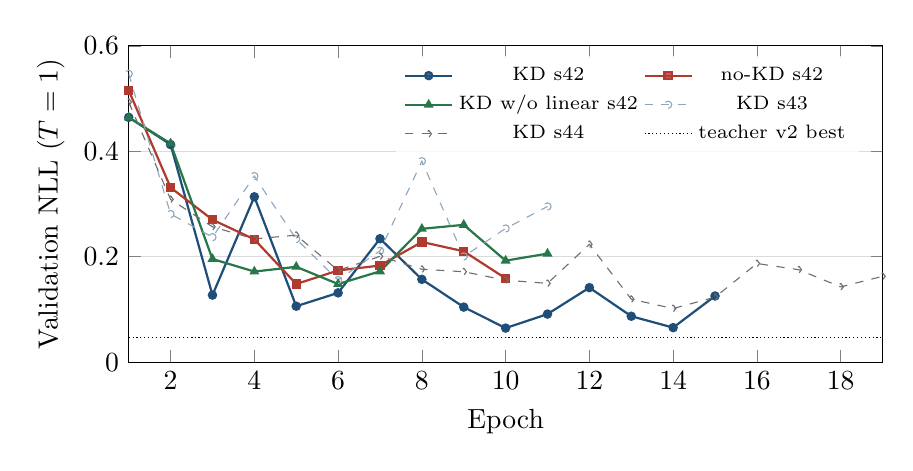
\begin{tikzpicture}
\begin{axis}[
  width=0.92\linewidth, height=5.6cm,
  xlabel={Epoch}, ylabel={Validation NLL ($T=1$)}, ymin=0, ymax=0.6, xmin=1, xmax=19,
  legend style={font=\scriptsize,draw=none,fill=white,fill opacity=0.8,text opacity=1}, legend pos=north east, legend columns=2,
  ymajorgrids, grid style={muted!25}, mark size=1.3pt]
\addplot[accent,thick,mark=*] coordinates {(1,0.4644)(2,0.4127)(3,0.1273)(4,0.3137)(5,0.1062)(6,0.1315)(7,0.2342)(8,0.1571)(9,0.1045)(10,0.0647)(11,0.0913)(12,0.1414)(13,0.0872)(14,0.0656)(15,0.1256)};
\addplot[warn,thick,mark=square*] coordinates {(1,0.5154)(2,0.3312)(3,0.2702)(4,0.2330)(5,0.1483)(6,0.1740)(7,0.1833)(8,0.2280)(9,0.2104)(10,0.1590)};
\addplot[okgreen,thick,mark=triangle*] coordinates {(1,0.4641)(2,0.4148)(3,0.1957)(4,0.1719)(5,0.1809)(6,0.1483)(7,0.1723)(8,0.2530)(9,0.2605)(10,0.1926)(11,0.2059)};
\addplot[accent!50,dashed,mark=o] coordinates {(1,0.5468)(2,0.2811)(3,0.2371)(4,0.3529)(5,0.2335)(6,0.1558)(7,0.2114)(8,0.3812)(9,0.2006)(10,0.2536)(11,0.2954)};
\addplot[muted,dashed,mark=diamond] coordinates {(1,0.4933)(2,0.3088)(3,0.2567)(4,0.2339)(5,0.2409)(6,0.1741)(7,0.2008)(8,0.1763)(9,0.1716)(10,0.1555)(11,0.1495)(12,0.2235)(13,0.1195)(14,0.1018)(15,0.1233)(16,0.1872)(17,0.1754)(18,0.1428)(19,0.1629)};
\addplot[black,thin,densely dotted,domain=1:19] {0.0472};
\legend{KD s42, no-KD s42, KD w/o linear s42, KD s43, KD s44, teacher v2 best}
\end{axis}
\end{tikzpicture}
\caption{Student validation NLL per epoch. The curves are noisy, and the best epoch per variant ranges from 5 to 14. The primary variant's best value (0.0647, epoch 10) is close to the teacher's (0.0472), while seed 43 reaches only 0.156.}
\label{fig:v12curves}
\end{figure}

% ----------------------------------------------------------------------------
\subsection{Deployment Runtime}
\label{sec:v12deploy}

The trained student is split at the boundary between sparse lookups and dense computation:
\begin{enumerate}
  \item \texttt{embeddings.npz}: $\bm E$, $\W_L$ and $\bb_L$, used from NumPy (\texttt{np.add.reduceat} computes \cref{eq:v12embed});
  \item \texttt{encoder.onnx}: positions, four blocks, pooling and head. Inputs are $\bm X\in\R^{1\times T\times256}$ and the mask; outputs are $\z^{\text{enc}}$ and $\bm\alpha$. Opset 17 with a dynamic token axis;
  \item \texttt{encoder.int8.onnx}: ONNX Runtime dynamic quantization (INT8 weights, dynamic activation scales), 12.8\,MB$\to$3.4\,MB;
  \item \texttt{meta.json}: configuration and calibration fitted on the \emph{deployed INT8 model's} validation logits.
\end{enumerate}
Across all evaluation messages, the maximum absolute logit difference between PyTorch and ONNX (fp32) is $5.8\times10^{-6}$. INT8 changes no intent prediction and one of 190 test sentiment predictions. One exporter pitfall was found and fixed: exporting through a wrapper module restores the wrapper's training flag \emph{recursively}, which had silently re-enabled dropout during the parity check (a 0.29 logit difference before the fix). \texttt{python v12/predict.py "text"} returns the same JSON as \texttt{solution.py predict}, optionally with $\bm\alpha$.

\subsubsection{Latency}
The hardware is an Apple M2 (Python 3.12, NumPy 2.3.5, ONNX Runtime 1.30), using the protocol of \cref{tab:latency}: 80 warm-up and 600 timed calls, batch 1, warm and serial. Each call includes hashing, the embedding mean, the encoder, the linear branch, calibration and JSON serialization.

\begin{table}[h]
\centering\small
\caption{Latency of the trained student by precision and ONNX Runtime intra-op threads (ms).}
\label{tab:v12latency}
\begin{tabular}{@{}l ccc ccc r@{}}
\toprule
& \multicolumn{3}{c}{Test messages} & \multicolumn{3}{c}{p95 by input length (code points)} & \\
\cmidrule(lr){2-4}\cmidrule(lr){5-7}
Configuration & p50 & p95 & p99 & 32 & 128 & 512 & Msg/s \\
\midrule
INT8, 1 thread  & 0.64 & 0.92 & 1.15 & 0.55 & 1.68 & 5.98 & 1{,}497 \\
\textbf{INT8, 2 threads} & \textbf{0.57} & \textbf{0.81} & \textbf{0.90} & 0.49 & 1.31 & \textbf{4.29} & 1{,}686 \\
INT8, 4 threads & 0.53 & 0.77 & 0.95 & 0.49 & 1.30 & 3.45 & 1{,}782 \\
FP32, 1 thread  & 1.14 & 1.62 & 1.75 & 0.90 & 2.98 & 10.96 & 867 \\
FP32, 2 threads & 0.81 & 1.14 & 1.23 & 0.68 & 1.97 & 6.83 & 1{,}201 \\
FP32, 4 threads & 0.68 & 1.00 & 1.39 & 0.61 & 1.65 & 4.91 & 1{,}388 \\
\midrule
v1.1, same machine & 0.27 & 0.38 & 0.45 & 0.25 & 0.55 & 1.40 & -- \\
\bottomrule
\end{tabular}
\end{table}

At 512 code points (106 tokens, 920 pieces), the encoder takes about 4.3\,ms of the 6.0\,ms single-thread total. The rest is hashing (0.30\,ms token pieces, 0.80\,ms v1.0 features) and the embedding mean (0.30\,ms). Two threads keep p95 below 5\,ms. Four threads were noisy on the M2's mixed performance and efficiency cores (3.45 to 5.10\,ms across three measurements), and p99 at 512 code points exceeded 5\,ms in an earlier thread sweep. The runtime therefore defaults to two threads. v1.1 remains two to three times faster (0.38 versus 0.81\,ms on test messages; 1.40 versus 4.29\,ms at 512 code points).

\subsubsection{Hosted Service}
\label{sec:v12hosted}

The same runtime backs a public deployment at
\url{https://polyglots-shorthand.onrender.com/}. A FastAPI process loads the
INT8 student once at start-up and exposes \texttt{GET /api/meta} (the
selectable models with their parameter counts, feature modes, test accuracy,
temperatures and review thresholds), \texttt{POST /api/predict} (up to 200
messages per request, with an optional \texttt{model} key) and generated API
documentation at \texttt{/api/docs}. The v1.1 checkpoints are loaded lazily on
first selection and then cached, so a session that never leaves the default
holds only the student's 36\,MB of weights.

Nothing in the service is specific to the host. It needs no environment
variables, no database and no external API, because the checkpoints are
committed to the repository and inference is NumPy plus ONNX Runtime. The
published instance is a 512\,MB free tier, which holds all five models at
once and suspends after inactivity; a request that wakes a suspended instance
waits for the container start and the ONNX session load, measured once at
32.5\,s, after which per-message latency returns to \cref{tab:v12latency}. All
timings reported in this paper are local and are unaffected by the host.

% ----------------------------------------------------------------------------
\subsection{Results}
\label{sec:v12results}

\begin{table}[t]
\centering\small
\caption{v1.2 development-test results (190 rows, 44 groups): macro-F1 with 95\% group-bootstrap interval and paired difference against v1.1 on identical resamples. Compare \cref{tab:v11main}.}
\label{tab:v12main}
\setlength{\tabcolsep}{3.2pt}
\resizebox{\linewidth}{!}{%
\begin{tabular}{@{}l r cc cc c cc c c@{}}
\toprule
& & \multicolumn{2}{c}{Intent} & \multicolumn{2}{c}{Sentiment} & Pos. & \multicolumn{2}{c}{Stress F1 (consistency)} & Emoji & Audit \\
\cmidrule(lr){3-4}\cmidrule(lr){5-6}\cmidrule(lr){8-9}
System & Params & F1 [95\% CI] & $\Delta$ vs v1.1 & F1 [95\% CI] & $\Delta$ vs v1.1 & recall & Intent & Sent. & pairs & err. \\
\midrule
v1.1 full & 0.83M &.901 [.78,.97] & -- &.845 [.72,.94] & -- &.72 &.865 (97.4\%) &.826 (92.6\%) & 9/12 & 6 \\
Teacher (v1.1 data) & 278M &.929 [.82, 1.00] & $+.032$ [$-.06$, $+.14$] & 1.000 [1.00, 1.00] & $\mathbf{+.159}$ [$+.06$, $+.28$] & 1.00 &.852 (92.6\%) & 1.000 (100\%) & 12/12 & 1 \\
Teacher v2 & 278M & \textbf{.966} [.92,.99] & $+.071$ [$-.007$, $+.172$] & 1.000 [1.00, 1.00] & $\mathbf{+.159}$ [$+.06$, $+.28$] & 1.00 & \textbf{.933} (95.8\%) & 1.000 (100\%) & 12/12 & 1 \\
\midrule
Student $+$ KD (s42) & 11.88M &.914 [.81,.98] & $+.014$ [$-.10$, $+.13$] &.911 [.82,.98] & $+.068$ [$-.07$, $+.21$] & 1.00 &.914 (97.9\%) &.917 (96.3\%) & 12/12 & 2 \\
Student no-KD (s42) & 11.88M &.888 [.77,.97] & $-.011$ [$-.12$, $+.11$] &.878 [.77,.96] & $+.034$ [$-.07$, $+.14$] &.93 &.895 (96.8\%) &.836 (92.6\%) & 12/12 & 3 \\
Student $+$ KD w/o linear (s42) & 11.58M &.958 [.89,.99] & $+.062$ [$-.03$, $+.17$] &.909 [.81,.98] & $+.066$ [$-.04$, $+.17$] &.93 &.918 (94.7\%) &.925 (96.3\%) & 11/12 & 1 \\
Student $+$ KD (s43) & 11.88M &.911 [.82,.98] & $+.014$ [$-.09$, $+.14$] &.853 [.74,.94] & $+.009$ [$-.11$, $+.13$] &.95 &.910 (98.9\%) &.813 (88.9\%) & 12/12 & 3 \\
Student $+$ KD (s44) & 11.88M &.919 [.82,.98] & $+.020$ [$-.09$, $+.13$] &.952 [.87, 1.00] & $+.110$ [$-.00$, $+.23$] &.93 &.914 (97.9\%) &.925 (97.4\%) & 12/12 & 1 \\
\textbf{Student $+$ KD, ONNX INT8 (deployed)} & 11.88M &.914 [.81,.98] & $+.014$ [$-.10$, $+.13$] &.916 [.83,.98] & $+.073$ [$-.06$, $+.22$] & 1.00 &.914 (97.9\%) &.917 (95.8\%) & 12/12 & 2 \\
\bottomrule
\end{tabular}}
\end{table}

\begin{figure}[t]
\centering
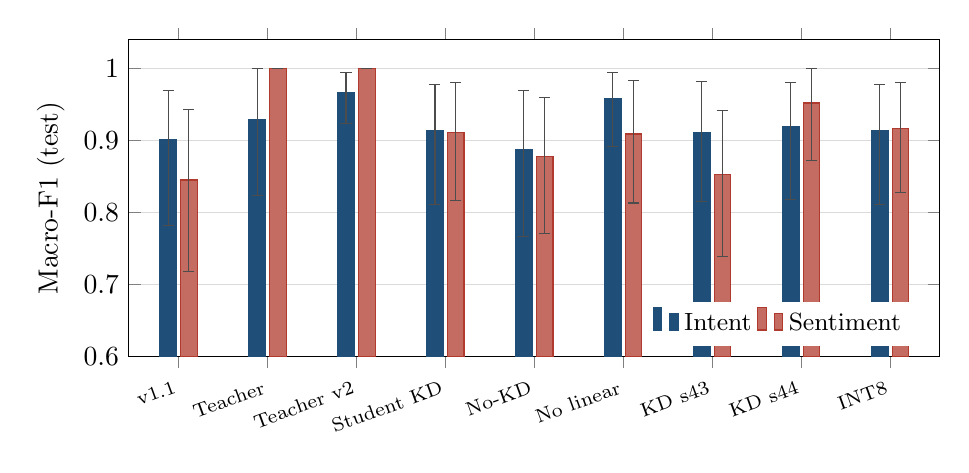
\begin{tikzpicture}
\begin{axis}[
  ybar=1.5pt, width=0.98\linewidth, height=5.6cm,
  ymin=0.6, ymax=1.04, ylabel={Macro-F1 (test)},
  symbolic x coords={v1.1,Teacher,Teacher v2,Student KD,No-KD,No linear,KD s43,KD s44,INT8},
  xtick=data, xticklabel style={font=\scriptsize,rotate=20,anchor=north east},
  enlarge x limits=0.07, bar width=6pt,
  legend style={font=\small,draw=none}, legend columns=2, legend pos=south east,
  ymajorgrids, grid style={muted!25},
  error bars/y dir=both, error bars/y explicit, error bars/error bar style={thin,black!70}]
\addplot[fill=accent,draw=accent] coordinates {
  (v1.1,0.901) += (0,0.069) -= (0,0.119)
  (Teacher,0.929) += (0,0.071) -= (0,0.106)
  (Teacher v2,0.966) += (0,0.028) -= (0,0.042)
  (Student KD,0.914) += (0,0.064) -= (0,0.103)
  (No-KD,0.888) += (0,0.081) -= (0,0.121)
  (No linear,0.958) += (0,0.037) -= (0,0.066)
  (KD s43,0.911) += (0,0.071) -= (0,0.096)
  (KD s44,0.919) += (0,0.061) -= (0,0.101)
  (INT8,0.914) += (0,0.064) -= (0,0.103)};
\addplot[fill=warn!75,draw=warn] coordinates {
  (v1.1,0.845) += (0,0.098) -= (0,0.127)
  (Teacher,1.000) += (0,0.0) -= (0,0.0)
  (Teacher v2,1.000) += (0,0.0) -= (0,0.0)
  (Student KD,0.911) += (0,0.069) -= (0,0.095)
  (No-KD,0.878) += (0,0.082) -= (0,0.107)
  (No linear,0.909) += (0,0.074) -= (0,0.096)
  (KD s43,0.853) += (0,0.089) -= (0,0.114)
  (KD s44,0.952) += (0,0.048) -= (0,0.080)
  (INT8,0.916) += (0,0.065) -= (0,0.088)};
\legend{Intent, Sentiment}
\end{axis}
\end{tikzpicture}
\caption{v1.2 test macro-F1 with 95\% group-bootstrap intervals (exact bootstrap percentiles). The teachers' sentiment is at the ceiling; every student interval overlaps v1.1.}
\label{fig:v12bars}
\end{figure}

\begin{table}[t]
\centering
\small
\setlength{\tabcolsep}{4pt}

\caption{Paired differences on the same 5,000 resamples: data ablation,
distillation gap and student ablations.}
\label{tab:v12paired}

\begin{tabularx}{\linewidth}{
    @{}
    >{\raggedright\arraybackslash}X
    >{\centering\arraybackslash}p{1.55cm}
    >{\centering\arraybackslash}p{2.35cm}
    >{\centering\arraybackslash}p{1.25cm}
    >{\centering\arraybackslash}p{1.55cm}
    >{\centering\arraybackslash}p{2.35cm}
    >{\centering\arraybackslash}p{1.25cm}
    @{}
}
\toprule

& \multicolumn{3}{c}{\textbf{Intent}}
& \multicolumn{3}{c}{\textbf{Sentiment}}
\\

\cmidrule(lr){2-4}
\cmidrule(lr){5-7}

\textbf{Comparison}
& $\overline{\Delta}$ [95\% CI]
& $P(\Delta>0)$
& 
& $\overline{\Delta}$ [95\% CI]
& $P(\Delta>0)$
&
\\

\midrule

Data: teacher v2 $-$ teacher (v1.1 data)
&
$+0.040$
&
$[-0.028,\,+0.121]$
&
$0.85$
&
$0.000$
&
$[0.000,\,0.000]$
&
$-$
\\

Distillation gap: student + KD $-$ teacher v2
&
$-0.057$
&
$[-0.136,\,+0.004]$
&
$0.04$
&
$\mathbf{-0.092}$
&
$[-0.184,\,-0.020]$
&
$0.02$
\\

KD effect: student + KD $-$ no-KD (s42)
&
$+0.025$
&
$[-0.034,\,+0.113]$
&
$0.70$
&
$+0.034$
&
$[-0.055,\,+0.124]$
&
$0.74$
\\

Linear branch: with $-$ without (s42)
&
$-0.048$
&
$[-0.124,\,+0.014]$
&
$0.07$
&
$+0.002$
&
$[-0.091,\,+0.094]$
&
$0.53$
\\

Quantization: INT8 $-$ FP32 (s42)
&
$+0.000$
&
$[+0.000,\,+0.000]$
&
$-$
&
$+0.005$
&
$[+0.000,\,+0.017]$
&
$0.64$
\\

\bottomrule
\end{tabularx}

\vspace{0.35em}

\begin{minipage}{\linewidth}
\footnotesize
\textbf{Seed spread of student + KD} (seeds 42/43/44):
intent mean 0.915, sd 0.004; sentiment mean 0.906, sd 0.049.
Best validation NLL: 0.065, 0.156 and 0.102.
\end{minipage}

\end{table}
\begin{table}[h]
\centering\small
\caption{Contrast set per phenomenon: intent accuracy and sentiment accuracy over rows, and the number of pairs with both members fully correct. NS negation scope, NN neutral \hi{nahi}, NG negated negative, UA unseen affect ($^\dagger$ affect words present in generated training data).}
\label{tab:v12contrast}
\begin{tabular}{@{}l cc cc cc cc c@{}}
\toprule
& \multicolumn{2}{c}{NS} & \multicolumn{2}{c}{NN} & \multicolumn{2}{c}{NG} & \multicolumn{2}{c}{UA$^\dagger$} & Pairs \\
\cmidrule(lr){2-3}\cmidrule(lr){4-5}\cmidrule(lr){6-7}\cmidrule(lr){8-9}
System & int & sent & int & sent & int & sent & int & sent & (of 40) \\
\midrule
v1.1                      &.65 &.90 &.85 &.75 &.90 &.45 &.85 &.70 & 10 \\
Teacher (v1.1 data)       &.70 &.95 &.80 & 1.00 &.70 & 1.00 &.90 &.90 & 24 \\
Teacher v2                & \textbf{.90} &.90 & \textbf{.90} &.95 &.70 & 1.00 &.95 & 1.00 & \textbf{29} \\
Student $+$ KD (s42, INT8) &.80 &.85 &.90 &.85 &.75 &.65 &.85 &.85 & 17 \\
Student no-KD (s42)       &.70 &.85 &.90 &.85 &.80 &.65 &.80 &.95 & 18 \\
Student $+$ KD w/o linear &.85 &.85 &.90 &.90 &.65 &.70 &.85 &.95 & 20 \\
\bottomrule
\end{tabular}
\end{table}

\begin{table}[h]
\centering\small
\caption{Row-normalized test sentiment confusion matrices. Compare \cref{tab:v11confusion}(b).}
\label{tab:v12sentcm}
\begin{tabular}{@{}l ccc c ccc@{}}
\toprule
& \multicolumn{3}{c}{\textbf{v1.1}} && \multicolumn{3}{c}{\textbf{Student $+$ KD (INT8)}} \\
\cmidrule(lr){2-4}\cmidrule(lr){6-8}
True & neg & neu & pos && neg & neu & pos \\
\midrule
\lbl{negative} & \cm{55}{59} & \cm{2}{2} & \cm{3}{3} && \cm{52}{55} & \cm{3}{3} & \cm{6}{6} \\
\lbl{neutral}  & \cm{6}{7} & \cm{54}{58} & 0 && 0 & \cm{54}{58} & \cm{6}{7} \\
\lbl{positive} & \cm{10}{10} & \cm{7}{7} & \cm{43}{44} && 0 & 0 & \cm{60}{61} \\
\bottomrule
\end{tabular}
\end{table}

\begin{table}[h]
\centering\small
\caption{Calibration and selective prediction on test (temperature and review threshold fitted on validation). Compare \cref{tab:v11calib}.}
\label{tab:v12calib}
\begin{tabular}{@{}l cc cc cc cc@{}}
\toprule
& \multicolumn{2}{c}{Temperature} & \multicolumn{2}{c}{ECE} & \multicolumn{2}{c}{Coverage} & \multicolumn{2}{c}{Acc.\ on accepted} \\
\cmidrule(lr){2-3}\cmidrule(lr){4-5}\cmidrule(lr){6-7}\cmidrule(lr){8-9}
System & $T_I$ & $T_S$ & int & sent & int & sent & int & sent \\
\midrule
v1.1 & 0.550 & 1.316 &.082 &.106 &.953 &.753 &.906 &.951 \\
Teacher (v1.1 data) & 0.595 & 1.316 &.070 &.014 & 1.000 & 1.000 &.916 & 1.000 \\
Teacher v2 & 0.400$^\ast$ & 0.508 &.044 &.000 & 1.000 & 1.000 &.963 & 1.000 \\
Student $+$ KD (s42) & 0.400$^\ast$ & 0.755 &.070 &.048 & 1.000 & 1.000 &.921 &.911 \\
Student $+$ KD, INT8 & 0.400$^\ast$ & 0.755 &.070 &.045 & 1.000 & 1.000 &.921 &.916 \\
\bottomrule
\end{tabular}
\\[2pt]{\footnotesize $^\ast$ lower boundary of the temperature grid.}
\end{table}

\paragraph{Q3: does the student keep the teacher's gains} No, and the evidence (\cref{tab:v12main,tab:v12paired,tab:v12contrast}) points the same way throughout:
\begin{enumerate}
  \item \textbf{Distillation gap.} Sentiment is significantly below teacher v2 ($-0.092$ $[-0.184, -0.020]$) and intent trends below it ($P(\Delta>0)=0.04$). Against v1.1, the deployed student's gains ($+0.014$ intent, $+0.073$ sentiment) are not resolved. The student solves 17 contrast pairs against the teacher's 29.
  \item \textbf{KD is not shown to help.} Both point estimates over the no-KD student are positive ($+0.025$, $+0.034$) but unresolved, and smaller than the seed standard deviation of the primary variant's sentiment (0.049). The no-KD student even solves one more contrast pair.
  \item \textbf{The linear branch appears to hurt intent.} Without it, intent is 0.958 with 20 contrast pairs; keeping it scores $-0.048$ $[-0.124, +0.014]$ with $P(\Delta>0)=0.07$. The deployed model keeps the branch because it was the pre-specified primary variant, and a single seed does not justify switching. In v1.1 the small attention branch helped on top of the lexical model (\cref{tab:v11paired}); with a four-layer encoder and teacher signal, the lexical branch no longer appears to add to intent.
  \item \textbf{Instability across seeds.} Intent is stable (sd 0.004), but sentiment ranges from 0.853 to 0.952 and best validation NLL from 0.065 to 0.156.
  \item \textbf{Sentiment errors changed direction.} v1.1 missed positives (recall 0.72, 17 of 61 predicted negative or neutral). The student finds every positive (recall 1.00) but calls 13 negative or neutral messages positive (\cref{tab:v12sentcm}), including negated complaints such as \hi{bahut problem hui, refund time pe nahi aaya}. This suggests over-learning of the negated-negative $\Rightarrow$ positive pattern from the generated data.
  \item \textbf{What did improve.} Stability under unseen misspellings is at least v1.1's (intent consistency 97.9\% versus 97.4\%, stress F1 0.914 versus 0.865); emoji pairs are 12/12; positive recall is 1.00; the student solves 17 contrast pairs against v1.1's 10; and INT8 quantization is lossless on these sets.
  \item \textbf{Calibration.} Validation thresholds collapse to 0 for every v1.2 model, so the review flag never fires on this split. v1.1's sentiment head deferred 24.7\% of messages.
\end{enumerate}

% ----------------------------------------------------------------------------
\subsection{Qualitative Error Analysis}
\label{sec:v12errors}

\begin{table}[h]
\centering\small
\caption{Representative errors of the deployed student (INT8) and teacher v2.}
\label{tab:v12errors}
\begin{tabularx}{\linewidth}{@{}p{5.0cm} p{3.0cm} X@{}}
\toprule
Message (set) & Gold $\to$ predicted & Interpretation \\
\midrule
\hi{bahut problem hui, refund time pe nahi aaya} (contrast, student) &
sentiment \lbl{neg}$\to$\lbl{pos} &
\emph{Negation over-learned.} The generated \hi{koi problem nahi} / \hi{bina hassle} rows teach ``negative word $+$ \hi{nahi} $\Rightarrow$ positive''; here \hi{nahi} negates the refund arriving, not the problem. \\
\addlinespace
\hi{itni jhanjhat ke baad bhi order cancel nahi hua} (contrast, student) &
sentiment \lbl{neg}$\to$\lbl{pos} &
Same mechanism; the teacher gets it right. \\
\addlinespace
\hi{replacement mat bhejna, paise account mein wapas daal do} (contrast, student) &
intent \lbl{refund}$\to$\lbl{cancel} &
\emph{Scope.} The negated action is ignored, but the real request (\hi{paise wapas}) is routed to the wrong operational intent. \\
\addlinespace
\hi{delivery mein bahut deri hui, parcel teen din late aaya} (contrast, both) &
intent \lbl{feedback}$\to$\lbl{not\_rcv} &
\emph{Keyword routing}, shared by teacher and student: delay vocabulary implies \lbl{not\_received}. \\
\addlinespace
\hi{mujhe abhi delivery ka otp nahi mila, kaise milega} (contrast, teacher v2) &
intent \lbl{track}$\to$\lbl{not\_rcv} &
\hi{nahi mila} is the strongest cue for \lbl{not\_received} in all training data. \\
\addlinespace
\hi{delivery phir late ghatiya service} (audit, teacher v2 and every student) &
intent \lbl{track}$\to$\lbl{not\_rcv}/\lbl{feedback} &
A short message with no request verb; the audit label assumes a tracking request. \\
\bottomrule
\end{tabularx}
\end{table}

% ----------------------------------------------------------------------------
\subsection{Application}
\label{sec:v12app}
Two interfaces ship with the system, and both default to the deployed
student. Of the models with weights available locally, it is the most
accurate on both heads (test accuracy 92.1\% intent and 91.6\% sentiment,
against 90.5\% and 84.7\% for v1.1). It also has the highest validation
accuracy (100\% and 96.8\%), so the choice does not rest on test data alone.
Teacher v2 is more accurate (96.3\% and 100\%), but its 1.1\,GB weights were
not retained after pseudo-labelling and it is not deployable within the
latency budget. Both interfaces keep the four v1.1 checkpoints selectable, so
the ablations of \cref{sec:v11} can be inspected interactively, and both plot
the attention-pooling weights $\bm\alpha$ (\cref{eq:v12pool}) per token as in
v1.1.

\paragraph{Streamlit (\texttt{app.py}).} The original interface. A sidebar
drop-down selects the model and reports its test accuracy, parameter count,
feature mode and calibration constants.

\paragraph{Web (\texttt{web/}).} A single static page served by a small
FastAPI backend, added so that the system can be published as an ordinary web
service rather than a notebook tool (\cref{sec:v12hosted}). One picker selects
among the same five models and drives both modes of the page. For a single
message it shows the predicted intent and sentiment, the calibrated
confidence, the complete probability vector of each head, the human-review
flag and the shaded attention weights; batch mode accepts up to 200 messages
and exports the predictions as CSV. Switching models discards any displayed
result, so no output is left attributed to the wrong checkpoint. The page is
plain HTML, CSS and JavaScript with no build step, and the backend adds only
FastAPI and Uvicorn to the inference dependencies.

% ----------------------------------------------------------------------------
\subsection{Threats to Validity}
\begin{itemize}
  \item \textbf{Same generator.} The v1.1 test and audit sets, most training data, the generated messages and the contrast set were all written by LLMs, the last two by the same assistant. Gains may partly reflect matching the generator's style: generated data lift validation and test vocabulary coverage to about 0.94. Sentiment of 1.000 is a ceiling on this distribution.
  \item \textbf{Contrast vocabulary overlap.} 18 contrast affect words enter training through generated data; UA results after data enrichment are not evidence of generalisation.
  \item \textbf{Out-of-domain public data.} Political, cricket, movie and chit-chat tweets with visible label noise (teacher--gold agreement 0.71) and restrictive licenses; they are not redistributed.
  \item \textbf{Pseudo-label noise.} Sentiment soft labels on 50{,}000 unlabeled tweets come from a teacher trained on 4{,}000 such tweets and support data.
  \item \textbf{Seeds and power.} One seed per teacher. Three student seeds exist only for the primary variant; the KD and linear-branch ablations use a single seed and are smaller than the primary variant's sentiment standard deviation. The test split has 44 groups.
  \item \textbf{Free-GPU training.} Colab T4 sessions; teacher checkpoints omit optimizer moments (weights, schedule and RNG state are kept); at most three learning rates; no student hyper-parameter search; the public-only pre-fine-tuning stage was skipped.
  \item \textbf{No human data.} No real customer messages were available. The evaluator scores a \texttt{human\_test.jsonl} file separately if one is added.
\end{itemize}

% ---------------------------------------------------------------------------

% ============================================================================
\section{Conclusion}
\label{sec:conclusion}

A 295K-parameter, NumPy-only hashed linear model with Unicode-preserving,
multi-granular features classifies the intent of Romanized Hindi--English
support messages with 0.82 macro-F1 on a leakage-controlled development test
and 0.96 on a small independent audit, at sub-millisecond latency. It meets
the footprint and speed requirements with wide margin. Its sentiment head,
however, is not reliable: it misses every held-out positive message and every
sarcasm contrast pair, and its practical role is to route uncertain cases to
human review. The main lesson is methodological---group-level splitting and
cluster-bootstrap intervals reveal that apparent improvements from additional
feature channels are not statistically supported at this data scale---and the
clear next step is more and better-annotated data rather than a larger model.

\paragraph{Version 1.1.} Following that lesson, v1.1 first enriched the data
(213 seeds, 884 rows, positive affect in every intent) and then added a
532{,}800-parameter self-attention branch trained with hand-derived gradients.
Together they raise development-test macro-F1 to $0.901$ for intent and
$0.845$ for sentiment, with positive recall $0.72$, 9/12 sarcasm pairs and
$0.865$ intent F1 under unseen misspellings. All of this runs at 0.43\,ms p95
with 828K parameters. The data change accounts for most of the sentiment gain.
The attention branch adds a paired improvement of about $+0.04$ macro-F1 on
both heads and a clear gain in spelling robustness. Negation scope remains
unsolved, and a smaller audit regression shows that new data can introduce new
spurious cues. The next version should therefore again start with targeted
data rather than a larger model.

\paragraph{Version 1.2.} v1.2 tested that advice directly. A pretrained
Hinglish encoder trained on the same 536 v1.1 examples resolves sentiment on
every set (paired $+0.159$ $[+0.056, +0.282]$) but not intent. Targeted data
then raise the teacher's negation-scope intent accuracy on a hand-written
contrast set from 0.70 to 0.90, fix the long-standing \hi{cancel mat karna}
audit error and bring intent to 0.966, although the data effect on the 44-group
test is not statistically resolved. Distilling that teacher into an
11.88M-parameter hashed-piece Transformer meets the deployment constraints
(p95 0.81\,ms; 4.29\,ms at 512 code points; lossless INT8) and keeps v1.1's
robustness to unseen misspellings. It does \emph{not}, however, keep the
teacher's gains: its sentiment is significantly below the teacher's, its
improvements over v1.1 are not resolved, knowledge distillation is not shown
to help, and sentiment varies strongly across seeds. The lessons are
therefore twofold. Pretraining is what fixed sentiment, and targeted data are
what moved negation scope. Both conclusions now rest on synthetic evaluation
data written by the same kind of generator as the training data, so the next
step is a human-collected test set rather than another model.

% ============================================================================
\appendix
\section{Hyperparameters}
\label{app:hparams}
\begin{table}[h]
\centering
\small
\setlength{\tabcolsep}{5pt}
\renewcommand{\arraystretch}{1.15}

\begin{tabularx}{\linewidth}{@{}
    >{\raggedright\arraybackslash}p{0.27\linewidth}
    >{\raggedright\arraybackslash}X
@{}}

\toprule
\textbf{Setting} & \textbf{Value} \\
\midrule

Hash dimension $D$
& $2^{15}=32{,}768$ \\

Outputs $K$
& 9 (6 intent + 3 sentiment) \\

Max input length
& 512 code points (reject, never truncate) \\

Character $n$-gram orders
& 3, 4, 5 (boundary-padded) \\

Interaction caps
& 8 symbol tokens $\times$ 64 word tokens \\

Alias map / shorthand map / stress map
& 20 / 10 / 14 entries \\

Epochs
& 55 \\

Learning rate
& $0.6/(1+e/20)$; bias $\times 0.1$ \\

Weight decay
& $\W\gets0.999\,\W$ once per epoch \\

Class weighting
& $N/(K\cdot n_c)$ per head \\

Checkpoint criterion
& Minimum unweighted validation NLL \\

Temperature grid
& 30 log-spaced values in $[0.4,4.0]$ \\

Review rule
& Maximum coverage subject to $\ge 5$ accepted and $\ge 90\%$
validation accuracy; otherwise $1.01$ \\

Random seed
& 42 (split, shuffle, SGD order) \\

\midrule
\multicolumn{2}{@{}l}{\textbf{Added in v1.1 (attention branch)}} \\

Embedding buckets $B$ / width $d$
& $2^{14}=16{,}384$ / 32 \\

Max tokens $T_{\max}$
& 128 (attention branch only) \\

Token pieces
& Word, alias (F,S), char 3/4-grams (F,C,S) \\

Layers
& 1 single-head self-attention + residual + $\tanh$,
attention pooling \\

Initialization
& $\bm E\sim\mathcal N(0,0.1^2)$, $\bm P=\bm 0$,
$\bm W_{Q,K,V}\sim\mathcal N(0,1/d)$,
$\bm W_O,\bm u\sim\mathcal N(0,0.1^2)$,
$\bm W_{\text{out}}\sim\mathcal N(0,0.01^2)$; seed 0 \\

Optimizers
& Adam lr $10^{-4}$ (dense), sparse Adagrad lr $0.01$
($\bm E$), both $\times 1/(1+e/20)$ \\

Regularization
& Token dropout 0.2; dense decay $\times 0.99$ per epoch \\

Selection
& Minimum validation NLL over 11 settings (\cref{tab:v11grid}) \\

Augmentation
& $\le 5$ variants: original, shorthand, respelling (12),
both, opener (6) \\

Alias map
& 27 entries \\

\midrule
\multicolumn{2}{@{}l}{\textbf{Added in v1.2 (teachers)}} \\

Encoders (01)
& hing-roberta, hing-roberta-mixed, hing-bert, MuRIL;
lr $\in\{2,3,5\}\times10^{-5}$ \\

Encoder (02)
& hing-roberta-mixed; lr $\in\{3,5\}\times10^{-5}$ \\

Batch / epochs / patience
& 16 / 12 / 3 (01); 32 / 6 / 2 (02) \\

Schedule
& AdamW, wd 0.01, 10\% (01) or 6\% (02) warm-up,
linear decay, clip 1.0, fp16 \\

Pooling / max length
& Masked mean / 128 subwords \\

Public sentiment sample (02)
& 4,000 fixed seeded rows, intent loss masked \\

\midrule
\multicolumn{2}{@{}l}{\textbf{Added in v1.2 (student)}} \\

Pieces / buckets / width
& Word, alias, char 3/4-grams / $2^{15}$ / $d=256$ \\

Encoder
& 4 pre-LN blocks, 4 heads, GELU FFN 1024,
dropout 0.1, $T_{\max}=128$ \\

Linear branch
& v1.0 channels, $D=2^{15}$, zero init \\

Loss
& CE + 1.0 KD ($\tau=2$) + 0.1 consistency;
intent-KD mask $\max p\ge0.6$ on support rows \\

Optimizer
& AdamW lr $5\times10^{-4}$, wd 0.01, 5\% warm-up,
cosine, clip 1.0, fp16, batch 64 \\

Epoch composition
& 4,061 support + 4,000 public labeled + 8,000 pool
(re-sampled) \\

Regularization
& Token dropout 0.15; early stopping on validation NLL,
patience 5, $\le 30$ epochs \\

Seeds
& 42 (all variants); 43, 44 (student + KD) \\

Deployment
& ONNX opset 17, dynamic INT8 (ONNX Runtime 1.30),
2 intra-op threads \\

\bottomrule
\end{tabularx}
\end{table}

\section{Reproduction}
\label{app:repro}

\begin{lstlisting}
python3 -m venv.venv
.venv/bin/python -m pip install -r requirements.txt   # numpy==2.3.5
.venv/bin/python solution.py predict "refund kab milega bhai"
PYTHON=.venv/bin/python./run.sh   # data, 4 models, audit, 13 tests (v1.1)
# v1.1: interactive app with a model drop-down
.venv/bin/python -m pip install -r requirements-app.txt
.venv/bin/streamlit run app.py
# v1.2: web interface (FastAPI + static page) on http://localhost:8000
.venv/bin/python -m pip install -r requirements-web.txt
.venv/bin/uvicorn web.server:app --port 8000
\end{lstlisting}

\noindent v1.2 (\texttt{v12/}; GPU steps are Colab notebooks that run end to end):
\begin{lstlisting}
uv venv --python 3.12.venv-v12
uv pip install --python.venv-v12/bin/python -r v12/requirements-v12.txt
cd v12
make smoke        # CPU smoke test of every trainer, incl. disconnect + resume
make bundle       # notebooks + bundle.zip for Colab/Kaggle
# Colab T4: notebooks/01_teacher -> 02_teacher_kd -> 03_student ("Run all")
unzip -o 01_teacher_outputs.zip -d runs/01_teacher && make eval-teacher
unzip -o 02_teacher_kd_outputs.zip -d runs/02_teacher_kd && make teacher-v2
unzip -o 03_student_outputs.zip -d runs/03_student && make deploy
make compare      # results/phase5_table.md
python predict.py "cancel mat karna, bas track karke batao"
\end{lstlisting}

\noindent Example output:
\begin{lstlisting}
{"intent":    {"label": "refund",  "confidence": 0.9999, "review_required": false},
 "sentiment": {"label": "neutral", "confidence": 0.8672, "review_required": false}}
\end{lstlisting}

\noindent Module map: \texttt{model.py} (normalization, features, heads,
training, calibration, portable \texttt{.npz} I/O with schema check and
\texttt{allow\_pickle=False}); \texttt{make\_data.py} (seeds, group split,
augmentation); \texttt{solution.py} (CLI, evaluation, ablations, stress test,
benchmark); \texttt{audit.py} (frozen audit); \texttt{test\_solution.py}
(11 invariant tests in v1.0; 13 in v1.1, adding a finite-difference gradient
check, word-order sensitivity and loading of v1.0 checkpoints). v1.1 also adds
\texttt{app.py}, a Streamlit interface whose sidebar drop-down selects
\texttt{full.npz}, \texttt{strip\_symbols.npz}, \texttt{word\_only.npz} or
\texttt{char\_word.npz}, and which plots the pooling weights $\bm\alpha$.
v1.0 \texttt{.npz} files still load as linear-only models. v1.1 checkpoints
store the attention arrays under \texttt{att\_*} keys. v1.2 adds the
\texttt{v12/polyglot12} package (hashing copy, teacher and student trainers,
augmentation, near-duplicate index, evaluator, ONNX runtime),
\texttt{v12/predict.py}, a data card (\texttt{v12/data/DATA\_CARD.md}), and
\texttt{app.py} defaulting to the deployed student. The hosted interface of
\cref{sec:v12hosted} is \texttt{web/server.py} with \texttt{web/static/},
declared by \texttt{requirements-web.txt} and a \texttt{Procfile}; it is
started with \texttt{uvicorn web.server:app} and takes no configuration
beyond the port. Bootstrap intervals, ECE and collision statistics in
this paper were computed from the released checkpoints by a separate
read-only analysis script with bootstrap seed 0.

\end{document}
